% A LaTeX template for MSc Thesis submissions to 
% Politecnico di Milano (PoliMi) - School of Industrial and Information Engineering
%
% S. Bonetti, A. Gruttadauria, G. Mescolini, A. Zingaro
% e-mail: template-tesi-ingind@polimi.it
%
% Last Revision: October 2021
%
% Copyright 2021 Politecnico di Milano, Italy. NC-BY

\documentclass{Configuration_Files/PoliMi3i_thesis}

%------------------------------------------------------------------------------
%	REQUIRED PACKAGES AND  CONFIGURATIONS
%------------------------------------------------------------------------------

% CONFIGURATIONS
\usepackage{parskip} % For paragraph layout
\usepackage{setspace} % For using single or double spacing
\usepackage{emptypage} % To insert empty pages
\usepackage{multicol} % To write in multiple columns (executive summary)
\usepackage{multirow}
\usepackage{outlines}
\usepackage{lscape}
\setlength\columnsep{15pt} % Column separation in executive summary
\setlength\parindent{0pt} % Indentation
\raggedbottom  




% PACKAGES FOR TITLES
\usepackage{titlesec}
% \titlespacing{\section}{left spacing}{before spacing}{after spacing}
\titlespacing{\section}{0pt}{3.3ex}{2ex}
\titlespacing{\subsection}{0pt}{3.3ex}{1.65ex}
\titlespacing{\subsubsection}{0pt}{3.3ex}{1ex}
\usepackage{color}

% PACKAGES FOR LANGUAGE AND FONT
\usepackage[english]{babel} % The document is in English  
\usepackage[utf8]{inputenc} % UTF8 encoding
\usepackage[T1]{fontenc} % Font encoding
\usepackage[11pt]{moresize} % Big fonts

% PACKAGES FOR IMAGES
\usepackage{graphicx}
\usepackage{transparent} % Enables transparent images
\usepackage{eso-pic} % For the background picture on the title page
\usepackage{subfig} % Numbered and caption subfigures using \subfloat.
\usepackage{tikz} % A package for high-quality hand-made figures.
\usetikzlibrary{}
\graphicspath{{./Images/}} % Directory of the images
\usepackage{caption} % Coloured captions
\usepackage{xcolor} % Coloured captions
\usepackage{amsthm,thmtools,xcolor} % Coloured "Theorem"
\usepackage{float}

% STANDARD MATH PACKAGES
\usepackage{amsmath}
\usepackage{amsthm}
\usepackage{amssymb}
\usepackage{amsfonts}
\usepackage{bm}
\usepackage[overload]{empheq} % For braced-style systems of equations.
\usepackage{fix-cm} % To override original LaTeX restrictions on sizes

% PACKAGES FOR TABLES
\usepackage{tabularx}
\usepackage{longtable} % Tables that can span several pages
\usepackage{colortbl}
\usepackage{hhline}

% PACKAGES FOR ALGORITHMS (PSEUDO-CODE)
\usepackage{algorithm}
\usepackage{algorithmic}
\usepackage{listings}

% PACKAGES FOR REFERENCES & BIBLIOGRAPHY
\usepackage[colorlinks=true,linkcolor=black,anchorcolor=black,citecolor=black,filecolor=black,menucolor=black,runcolor=black,urlcolor=black]{hyperref} % Adds clickable links at references
\usepackage{cleveref}
\usepackage{hyperref}
\usepackage[square, numbers, sort&compress]{natbib} % Square brackets, citing references with numbers, citations sorted by appearance in the text and compressed
\bibliographystyle{abbrvnat} % You may use a different style adapted to your field

% OTHER PACKAGES
\usepackage{pdfpages} % To include a pdf file
\usepackage{afterpage}
\usepackage{lipsum} % DUMMY PACKAGE
\usepackage{fancyhdr} % For the headers
\fancyhf{}

% Input of configuration file. Do not change config.tex file unless you really know what you are doing. 
% Define blue color typical of polimi
\definecolor{bluepoli}{cmyk}{0.4,0.1,0,0.4}

% Custom theorem environments
\declaretheoremstyle[
  headfont=\color{bluepoli}\normalfont\bfseries,
  bodyfont=\color{black}\normalfont\itshape,
]{colored}

% Set-up caption colors
\captionsetup[figure]{labelfont={color=bluepoli}} % Set colour of the captions
\captionsetup[table]{labelfont={color=bluepoli}} % Set colour of the captions
\captionsetup[algorithm]{labelfont={color=bluepoli}} % Set colour of the captions

\theoremstyle{colored}
\newtheorem{theorem}{Theorem}[chapter]
\newtheorem{proposition}{Proposition}[chapter]

% Enhances the features of the standard "table" and "tabular" environments.
\newcommand\T{\rule{0pt}{2.6ex}}
\newcommand\B{\rule[-1.2ex]{0pt}{0pt}}

% Pseudo-code algorithm descriptions.
\newcounter{algsubstate}
\renewcommand{\thealgsubstate}{\alph{algsubstate}}
\newenvironment{algsubstates}
  {\setcounter{algsubstate}{0}%
   \renewcommand{\STATE}{%
     \stepcounter{algsubstate}%
     \Statex {\small\thealgsubstate:}\space}}
  {}

% New font size
\newcommand\numfontsize{\@setfontsize\Huge{200}{60}}

% Title format: chapter
\titleformat{\chapter}[hang]{
\fontsize{50}{20}\selectfont\bfseries\filright}{\textcolor{bluepoli} \thechapter\hsp\hspace{2mm}\textcolor{bluepoli}{|   }\hsp}{0pt}{\huge\bfseries \textcolor{bluepoli}
}

% Title format: section
\titleformat{\section}
{\color{bluepoli}\normalfont\Large\bfseries}
{\color{bluepoli}\thesection.}{1em}{}

% Title format: subsection
\titleformat{\subsection}
{\color{bluepoli}\normalfont\large\bfseries}
{\color{bluepoli}\thesubsection.}{1em}{}

% Title format: subsubsection
\titleformat{\subsubsection}
{\color{bluepoli}\normalfont\large\bfseries}
{\color{bluepoli}\thesubsubsection.}{1em}{}

% Shortening for setting no horizontal-spacing
\newcommand{\hsp}{\hspace{0pt}}

\makeatletter
% Renewcommand: cleardoublepage including the background pic
\renewcommand*\cleardoublepage{%
  \clearpage\if@twoside\ifodd\c@page\else
  \null
  \AddToShipoutPicture*{\BackgroundPic}
  \thispagestyle{empty}%
  \newpage
  \if@twocolumn\hbox{}\newpage\fi\fi\fi}
\makeatother

%For correctly numbering algorithms
\numberwithin{algorithm}{chapter}

%----------------------------------------------------------------------------
%	NEW COMMANDS DEFINED
%----------------------------------------------------------------------------

% EXAMPLES OF NEW COMMANDS
\newcommand{\bea}{\begin{eqnarray}} % Shortcut for equation arrays
\newcommand{\eea}{\end{eqnarray}}
\newcommand{\e}[1]{\times 10^{#1}}  % Powers of 10 notation

%----------------------------------------------------------------------------
%	ADD YOUR PACKAGES (be careful of package interaction)
%----------------------------------------------------------------------------

%----------------------------------------------------------------------------
%	ADD YOUR DEFINITIONS AND COMMANDS (be careful of existing commands)
%----------------------------------------------------------------------------

%----------------------------------------------------------------------------
%	BEGIN OF YOUR DOCUMENT
%----------------------------------------------------------------------------

\begin{document}

\fancypagestyle{plain}{%
\fancyhf{} % Clear all header and footer fields
\fancyhead[RO,RE]{\thepage} %RO=right odd, RE=right even
\renewcommand{\headrulewidth}{0pt}
\renewcommand{\footrulewidth}{0pt}}

%----------------------------------------------------------------------------
%	TITLE PAGE
%----------------------------------------------------------------------------

\pagestyle{empty} % No page numbers
\frontmatter % Use roman page numbering style (i, ii, iii, iv...) for the preamble pages

\puttitle{
	title=Simulation of a Humanoid Robot in Gazebo Environment, % Title of the thesis
	name=Giovanni Porcellato, % Author Name and Surname
	course=Automation and Control Engineering - Ingegneria dell'Automazione, % Study Programme (in Italian)
	ID  = 10745779,  % Student ID number (numero di matricola)
	advisor= Prof. Matteo Matteucci, % Supervisor name
		coadvisor={Simone Mentasti},
	academicyear={2021-22},  % Academic Year
} % These info will be put into your Title page 

%----------------------------------------------------------------------------
%	PREAMBLE PAGES: ABSTRACT (inglese e italiano), EXECUTIVE SUMMARY
%----------------------------------------------------------------------------
\startpreamble
\setcounter{page}{1} % Set page counter to 1

% ABSTRACT IN ENGLISH
\chapter*{Abstract} 
Here goes the Abstract in English of your thesis followed by a list of keywords.
The Abstract is a concise summary of the content of the thesis (single page of text)
and a guide to the most important contributions included in your thesis.
The Abstract is the very last thing you write.
It should be a self-contained text and should be clear to someone who hasn't (yet) read the whole manuscript.
The Abstract should contain the answers to the main scientific questions that have been addressed in your thesis.
It needs to summarize the adopted motivations and the adopted methodological approach as well as the findings of your work and their relevance and impact.
The Abstract is the part appearing in the record of your thesis inside POLITesi,
the Digital Archive of PhD and Master Theses (Laurea Magistrale) of Politecnico di Milano.
The Abstract will be followed by a list of four to six keywords.
Keywords are a tool to help indexers and search engines to find relevant documents.
To be relevant and effective, keywords must be chosen carefully.
They should represent the content of your work and be specific to your field or sub-field.
Keywords may be a single word or two to four words. 
\\
\\
\textbf{Keywords:} here, the keywords, of your thesis % Keywords

% ABSTRACT IN ITALIAN
\chapter*{Abstract in lingua italiana}
Qui va l'Abstract in lingua italiana della tesi seguito dalla lista di parole chiave.
\\
\\
\textbf{Parole chiave:} qui, vanno, le parole chiave, della tesi % Keywords (italian)

%----------------------------------------------------------------------------
%	LIST OF CONTENTS/FIGURES/TABLES/SYMBOLS
%----------------------------------------------------------------------------

% TABLE OF CONTENTS
\thispagestyle{empty}
\tableofcontents % Table of contents 
\thispagestyle{empty}
\cleardoublepage

%-------------------------------------------------------------------------
%	THESIS MAIN TEXT
%-------------------------------------------------------------------------
% In the main text of your thesis you can write the chapters in two different ways:
%
%(1) As presented in this template you can write:
%    \chapter{Title of the chapter}
%    *body of the chapter*
%
%(2) You can write your chapter in a separated .tex file and then include it in the main file with the following command:
%    \chapter{Title of the chapter}
%    \input{chapter_file.tex}
%
% Especially for long thesis, we recommend you the second option.

\addtocontents{toc}{\vspace{2em}} % Add a gap in the Contents, for aesthetics
\mainmatter % Begin numeric (1,2,3...) page numbering

% --------------------------------------------------------------------------
% NUMBERED CHAPTERS % Regular chapters following
% --------------------------------------------------------------------------
\chapter{Introduction}
\label{intro}
\section{Introduction}
In the field of robotics, platforms are of increasing importance. A platform is divided into a software platform and a hardware platform. There are a variety of features that make up robot software platforms, including low-level device control, SLAM (Simultaneous Localization and Mapping), navigation, manipulation, recognition of objects or people, sensing and package management, debugging and development tools, which are mostly used in the industrial sector where robot software platforms are currently primarily employed. Robot hardware platforms not only study platforms such as mobile robots, drones, and humanoids, but also commercial products. Hence, robot researchers from around the world are collaborating to discover a platform that is intuitive and open source. The most popular robot software platform is ROS, that means Robot Operating System. ROS, the Robot Operating System, is an open source framework to manage robots’ operations, tasks, motions, and other things. ROS is intended to serve as a software platform for those who build and use robots daily, but at the same time for people who are starting to use robots no long ago. This common platform allows newcomers to be increasingly inclined to read more and more and it is very easy to use. The design of the ROS platform allows the use of code and information shared by other programmers, which means you do not have to write all code in order to move the robots.
\newpage
\section{History of ROS}
“In May 2007, ROS was started by borrowing the early opensource robotic software frameworks including switchyard, which is developed by Dr. Morgan Quigley by the Stanford Artificial Intelligence Laboratory in support of the Stanford AI Robot STAIR (Stanford AI Robot) project.
Dr. Morgan Quigley is one of the founders and software development manager of Open Robotics (formerly the Open Source Robotics Foundation, OSRF), which is responsible for the development and management of ROS.
Switchyard is a program created for the development of artificial intelligence robots used in the AI lab’s projects at the time and it is the predecessor of ROS.
In addition, Dr. Brian Gerkey, the developer of the Player/Stage Project and 2D Stage simulator, later influence the growth of 3D simulator Gazebo, which was developed since 2000 and has had a major impact on ROS’s networking program. He is the co-founder of Open Robotics.
In November 2007, U.S. robot company Willow Garage succeeded the development of ROS. Willow Garage is a well-known company in the field of personal robots and service robots.” \cite{Quigley15}\\
Robots are computer-controlled electromechanical devices.
First dedicated robot programming languages arose in the 1970's.
There were robot-centric data types and some robot function libraries. They did not allow neither hardware abstractio, nor multi-robot interaction nor integrated simulation. There did not exist code reuse or standardization.
The efforts to build robot programming system continued through 80's, 90's and especially in the 2000's were there was a high push to standardize robot components, their interfaces and basic functions.\\
Hence, ROS as it is known today was initially developed in 2007 at the Standford Artificial Intelligence Laboratory. Since 2013 it is managed by OSRF and nowadays it is used by many robots, universities and companies, becoming the de facto standard for robot programming.
\begin{figure}[H]
    \centering
    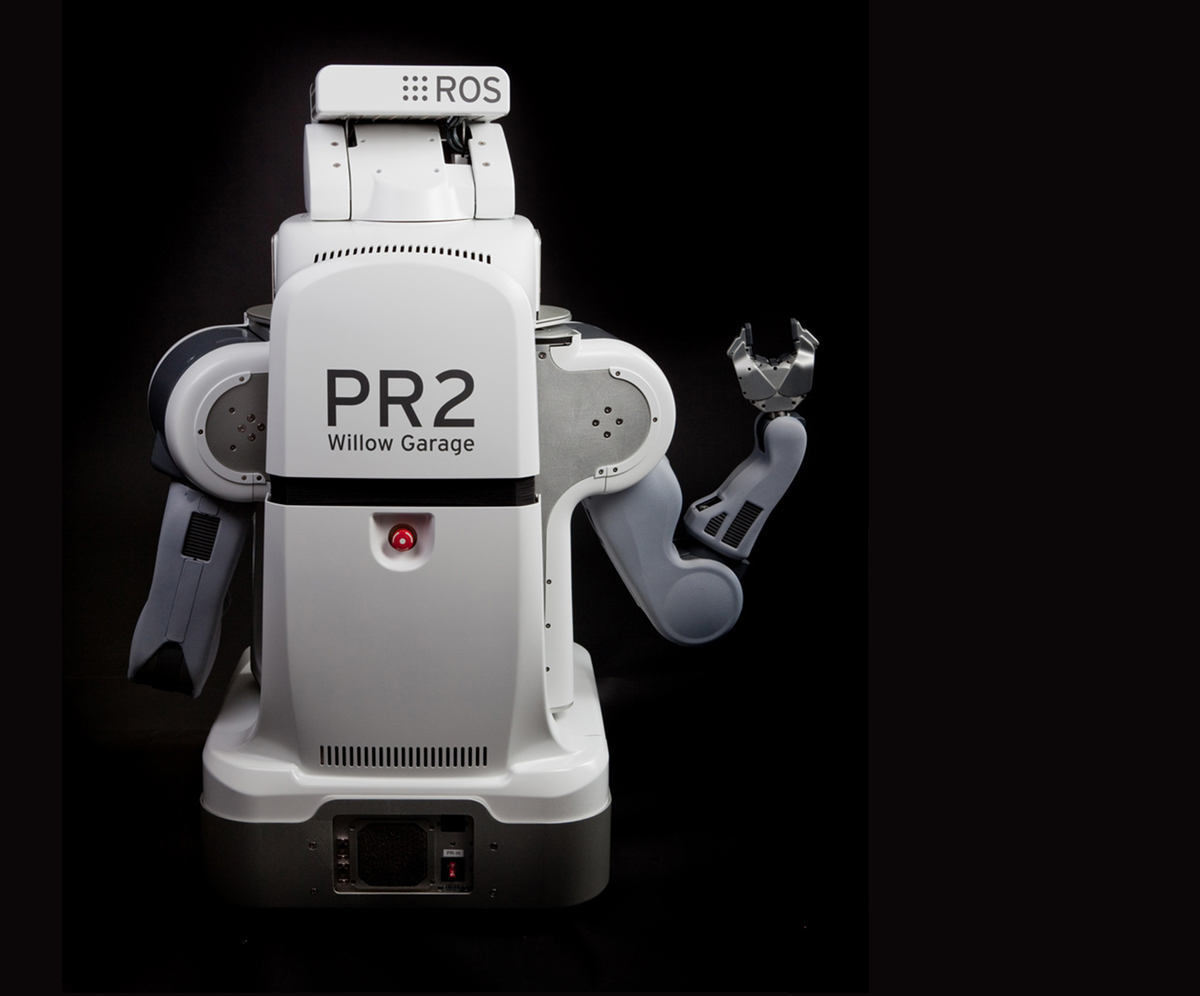
\includegraphics[scale=0.16]{Images/Chapter 1/PR2_Robot_Willow_Garage_6-1.jpeg}
    \caption{Willow Garage PR2 robot}
    \label{fig:PR2}
\end{figure}
\newpage
\section{Meta-Operating System}
ROS is an open source, meta operating framework for robots, hence it is nothing else than a middleware. \\
A middleware can be defined as a piece of software that gives an extra level of abstraction to the developer through a layer between the operating system and the applications.
It basically sits in the middle of software components and facilitates their interaction. \\
Its purpose is to provide an abstraction model for functions and at the same time provides the low-level implementation.
Every middleware must provide:
\begin{itemize}
    \item Portability: common programming model regardless the programming language and system architecture
    \item Complexity management: low-level aspects are managed by libraries and drivers inside the middleware itslef
    \item Reliability: middleware allows robot developer to discard low level details
    \item abstraction from sensors/actuators hardware;
    \item communication protocol for data transport
\end{itemize}
 As a result, they play an essential role in the development of complex applications that rely on a number of hardware and software tools.\\
 While they are still under active development, they are not yet capable of providing a complete set of functions for general purpose robots.
 
\begin{figure}[H]
    \centering
    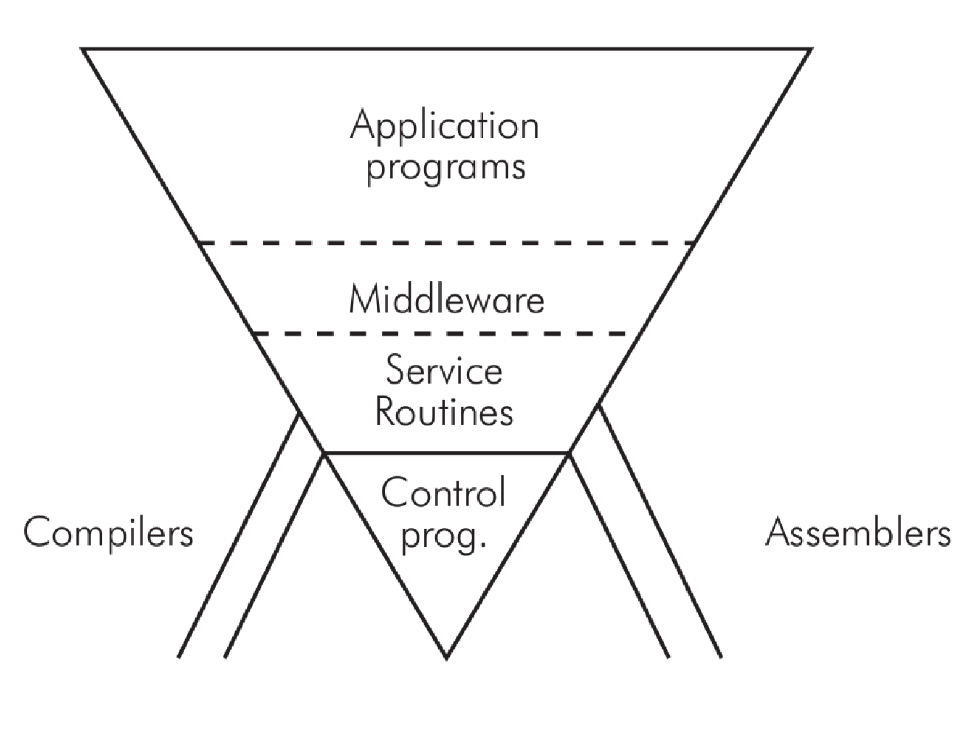
\includegraphics[scale=0.5]{Images/Chapter 1/middleware.png}
    \caption{Meta Operating System}
    \label{fig:metaoperating}
\end{figure}
 
 Several robotic middlewares have been proposed in the past years (OROCOS, ORCA, YARP, BRICS etc.) and eventually came ROS.
 
 \subsection{Phylosophy of ROS}
The following paragraphs describe some philosophical aspects of ROS:\\
\begin{itemize}
\item \textit{Peer to peer}: ROS systems consist of a small number of computer programs that are linked to one another and continuously exchange messages. These messages travel directly from one program to another. Although this makes the system more complex, the result is a system that balances better as the number of data increases.\\
\item \textit{Distributed}: Programs can be run on multiple computers and comunicate over the network.
\item \textit{Multilingual}: ROS chose a multilingual approach. ROS software modules can be written in any language for which a client library has been written. At the time of writing, client libraries exist for C++, Python, LISP, Java, JavaScript, MATLAB and others.\\
\item \textit{Thin}: the ROS conventions encourage contributors to create standalone libraries and then wrap those libraries, so that they can send and receive messages to and from other ROS modules. This extra layer is proposed to allow the reuse of software outside of ROS for other applications, and it greatly simplifies the creation of automated tests using standard continuous integration tools.\\
\item \textit{Free and open source}: the core of ROS is released under the permissive BSD license, which allows both commercial and non-commercial use. ROS foresees data exchange between modules using inter-process communication (IPC), which means that systems built using ROS can have fine-grained licensing of their various components.\\
\end{itemize}

\section{ROS Architecture}
ROS is based on a graph architecture where processing takes place in nodes, which communicate with each other by exchanging messages asynchronously through the use of topics to which they can subscribe to and/or on which they can publish, and synchronously with the calling of services, similar to RPCs.  Structurally, ROS is developed on 3 conceptual levels, File-system Level, Computational Level and Community Level, of which we are going to examine the constituent elements and their role in the architecture.
\subsection{File-system Level}
The Filesystem Level includes all resources used in ROS, in particular
\begin{itemize}
    \item Packages
    \item Metapackages
    \item Manifest
    \item Message types
    \item Service types
\end{itemize}
\begin{figure}
    \centering
    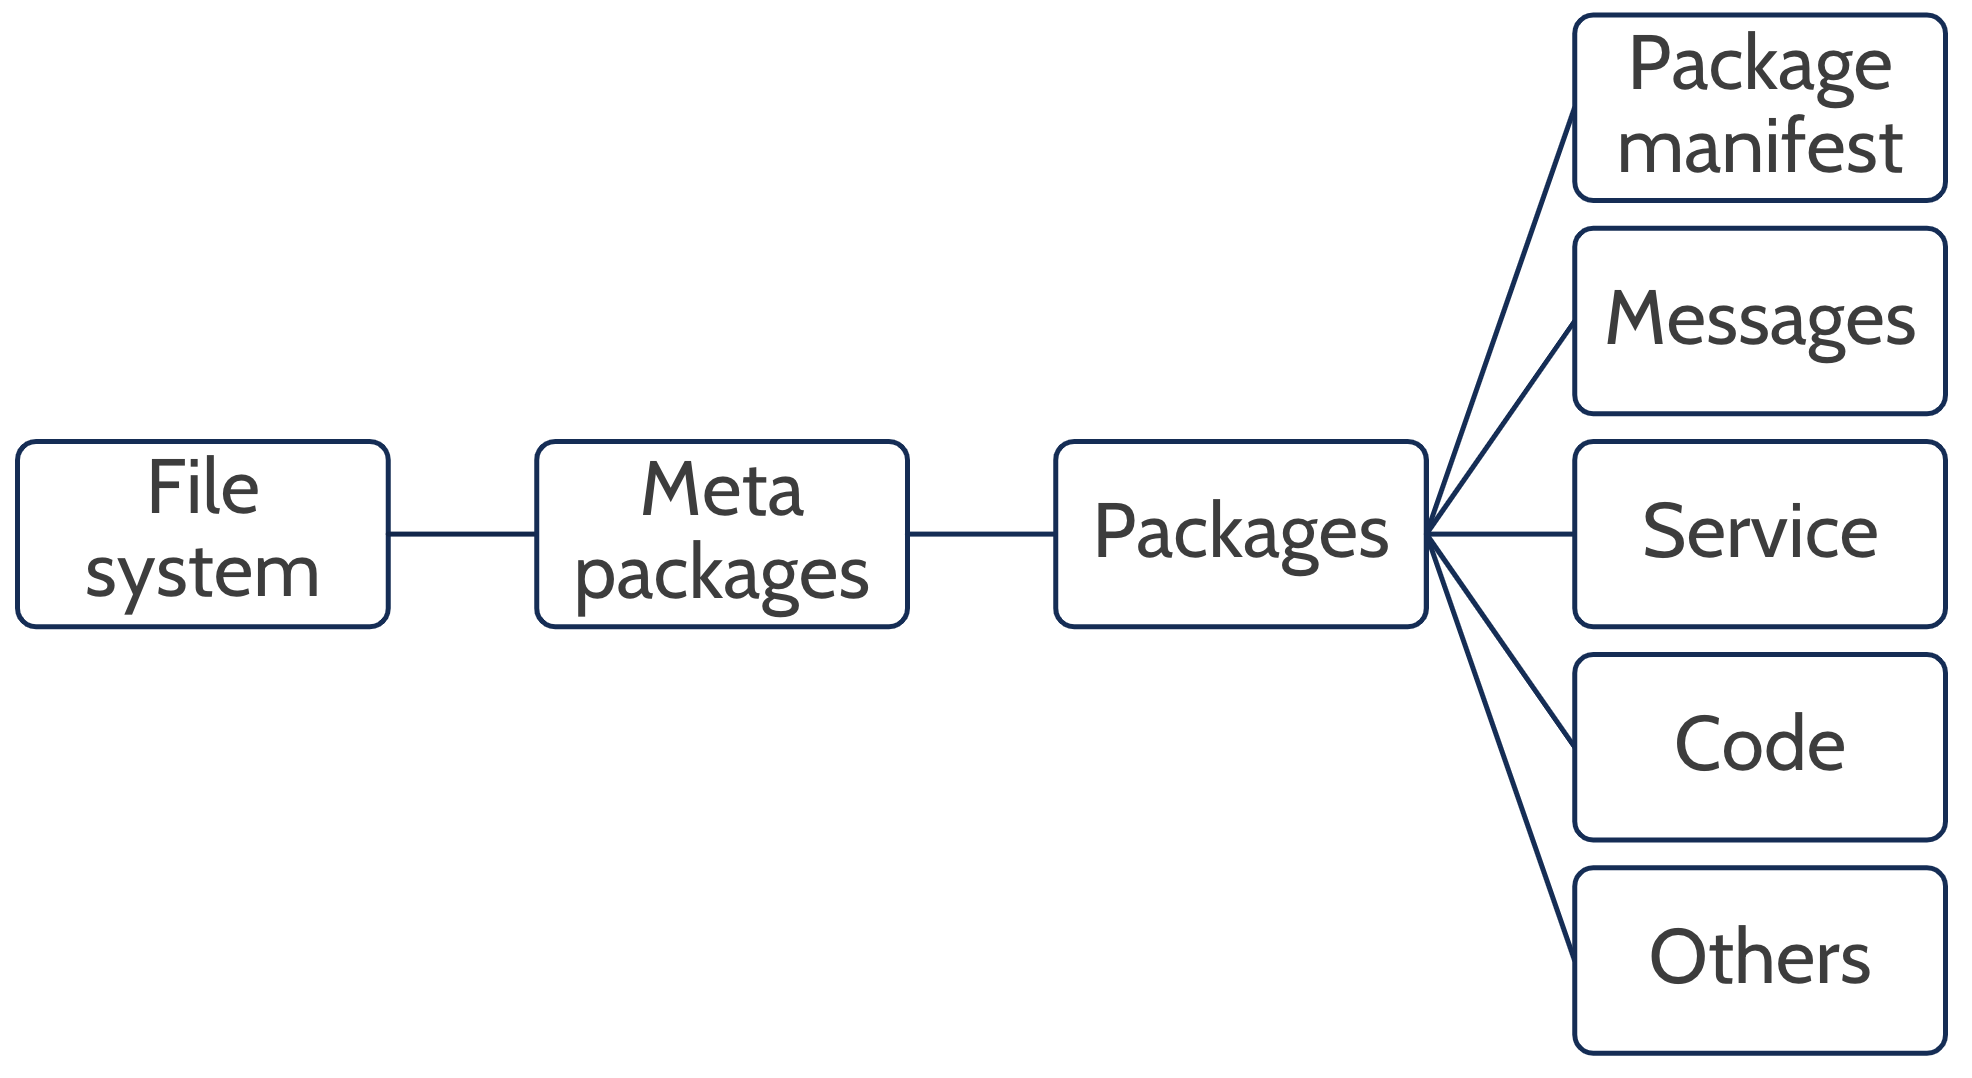
\includegraphics[scale=0.5]{Images/Chapter 1/Filesystem.png}
    \caption{File System level representation}
    \label{fig:Filesystem}
\end{figure}
\textbf{Packages}\\
Packages are the main structure for organising ROS  \citet{rospackages}. The processes, libraries, configuration files, datasets, and all the files used by the system at runtime are stored in these files. They are the structure that can be found within a ROS-based system. At the filesystem level, the package is represented by a directory. The structure within it includes some subfolders to manage the elements
In order to facilitate its development, in particular:
\begin{itemize}
    \item \textit{include/packagename}: C++ include headers (make sure to export in the CMakeLists.txt)
    \item \textit{msg}:Folder containing Message (msg) types
    \item \textit{src/packagename}: Source files, especially Python source that are exported to other packages.
    \item \textit{srv/}: Folder containing Service (srv) types
    \item \textit{scripts}: executable scripts
    \item \textit{CMakeLists.txt}: CMake build file
    \item \textit{package.xml}:XML file containing package structure 
    \item \textit{CHANGELOG.rst}: Many packages will define a changelog which can be automatically injected into binary packaging and into the wiki page for the package
\end{itemize}\\

\textbf{Metapackages}\\
Metapackages are specialised structures whose only task is to represent a group of packages that have common characteristics with each other. The metapackages that are created in the context of older versions of ROS and later updated may also result from the conversion of older stacks that perform similar functions in the context of older versions of ROS \citet{rosmetapackages}.\\
\newline
\textbf{Manifest}\\
A package manifest consists of an XML file named package.xml that must be included in the root folder of any catkin-compliant package. It contains information about the package, including its name, version number, authors, maintainers, and dependencies on other catkin packages. There is a strong similarity between this concept and the manifest.xml file used in the legacy rosbuild build system. System package dependencies are declared in package.xml \citet{rosmanifest}.\\
\newpage
There are a minimal set of tags that need to be nested within the <package> tag to make the package manifest complete.
\begin{itemize}
    \item \textit{<name>}: The name of the package
    \item \textit{<version>}: The version number of the package;
    \item \textit{<description>}: A description of the package contents;
    \item \textit{<maintainer>}: The name of the person(s) that is/are maintaining the package;
    \item \textit{<license}: The software license under which the code is released.
\end{itemize}
\textbf{Message types}\\
Message types define the structure of messages sent by ROS \citet{rosmsg}. Each file, with extension .msg, represents a different type of message. Within the file each line represents a message field. Each line, in turn, contains two columns: the first one for the data type of the field
(Int32/int (C++/Phyton), bool, string, time, etc.), the second for the name. It is possible to assign values to the fields within these le, in this case we speak of constants. Example of msg file (C++):

\textbf{Service types}\\
Service type are files that define the structure of request/response for ROS services \citet{rossrv}.
These are directly built upon the msg format to enable communication between nodes. They are stored in dedicated .srv files in the srv/ subdirectory of a package.
Example of srv file (C++):
\begin{lstlisting}[language=C++]
 bool add(beginner_tutorials::AddTwoInts::Request  &req,
             beginner_tutorials::AddTwoInts::Response &res)
    {
      res.sum = req.a + req.b;
      ROS_INFO("request: x=%ld, y=%ld", (long int)req.a, (long int)req.b);
      ROS_INFO("sending back response: [%ld]", (long int)res.sum);
     return true;
   }
\end{lstlisting}

\newpage

\subsection{ROS Computational Graph Level}
The Computation Graph is the peer-to-peer network of ROS processes that are processing data together. The basic Computation Graph concepts of ROS are nodes, Master, Parameter Server, messages, services, topics, and bags, all of which provide data to the Graph in different ways \citet{rosconcepts}.\\
\begin{figure}[H]
    \centering
    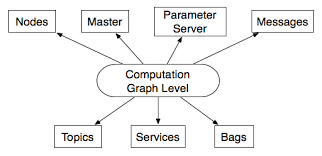
\includegraphics{Images/Chapter 1/computationgraph.png}
    \caption{Computation Graph}
    \label{fig:computationgraph}
\end{figure}
\textbf{Nodes}\\
A node is a process that performs computation. Nodes are combined together into a graph and communicate with one another using streaming topics, RPC services, and the Parameter Server \citet{rosnodes}. Following the concept of modularity of the system, each node will be related to only one specific functionality.\\ ROS in fact
discourages the creation of 'omnipotent' nodes that perform many functions in order to make the system more maintainable, reusable and clear.\\
The use of nodes in ROS provides several benefits to the overall system. There is additional fault tolerance as crashes are isolated to individual nodes. Code complexity is reduced in comparison to monolithic systems.\\
\newpage
\textbf{Topics}\\
Topics are buses identified by a proper and unique name that allow messages to be exchanged between nodes. They implement a mechanism
of publishing and subscribing: nodes can be publishers and/or subscribers if they are set up to send or receive messages. The division between
data producer and data user is clear and separated by anonymity policies
between the nodes. Each topic may have a maximum number of messages to be kept
in the queue in case they accumulate, those in excess are not added to the queue and lost \citet{rostopics}.\\
\newline
\textbf{Services}\\
Services are a two-way communication tool between nodes. It is a mechanism that extends that of messages with the possibility
not only to send commands to a specific node but also to remain in
listening and receiving a structured response from it. Each service is
first described in an .srv file where the parameters and type of service are indicated in addition to the name of the service.
of the service, as well as the parameters and the type of return data (see Service type).
Within the server node, the service is represented by a function
which takes as input two pointers to objects of the server class: one
one will include the function parameters (Request), the other will collect the return value.
will collect the return value \citet{rosservice}\\
\newline
\textbf{Messages}\\
The nodes in the graph communicate by exchanging messages. These
may be simple and of a primitive type (integer 
oat, string, char, etc.)
or arrays or even more complex, with structures similar to those seen in
C.\\
\newline
\textbf{Bags}\\
Bags represent the system by which ROS saves logs and keeps track of
all messages exchanged within a topic. The rosbag tool, once
associated with a topic, saves each message exchanged within a related file with the extension .bag. It is
very useful for storing data from the
sensors as it allows the developer to create a sort of "black box" of the robot.
black box" of the robot. ROS also provides a playback tool that allows the
visualise and playback the collected data via a graphical interface.\\
\newpage
\textbf{Master}\\
The master in ROS first takes care of registering new nodes within the
network, then managing the connection between the nodes in the graph, routing
messages and allowing access by one node to the services of another.
It is the heart of the software and can only be active one master at a time. It can be started via the roscore command or launched automatically
at the start of a node through the correct implementation of the file.
\begin{figure}[H]
    \centering
    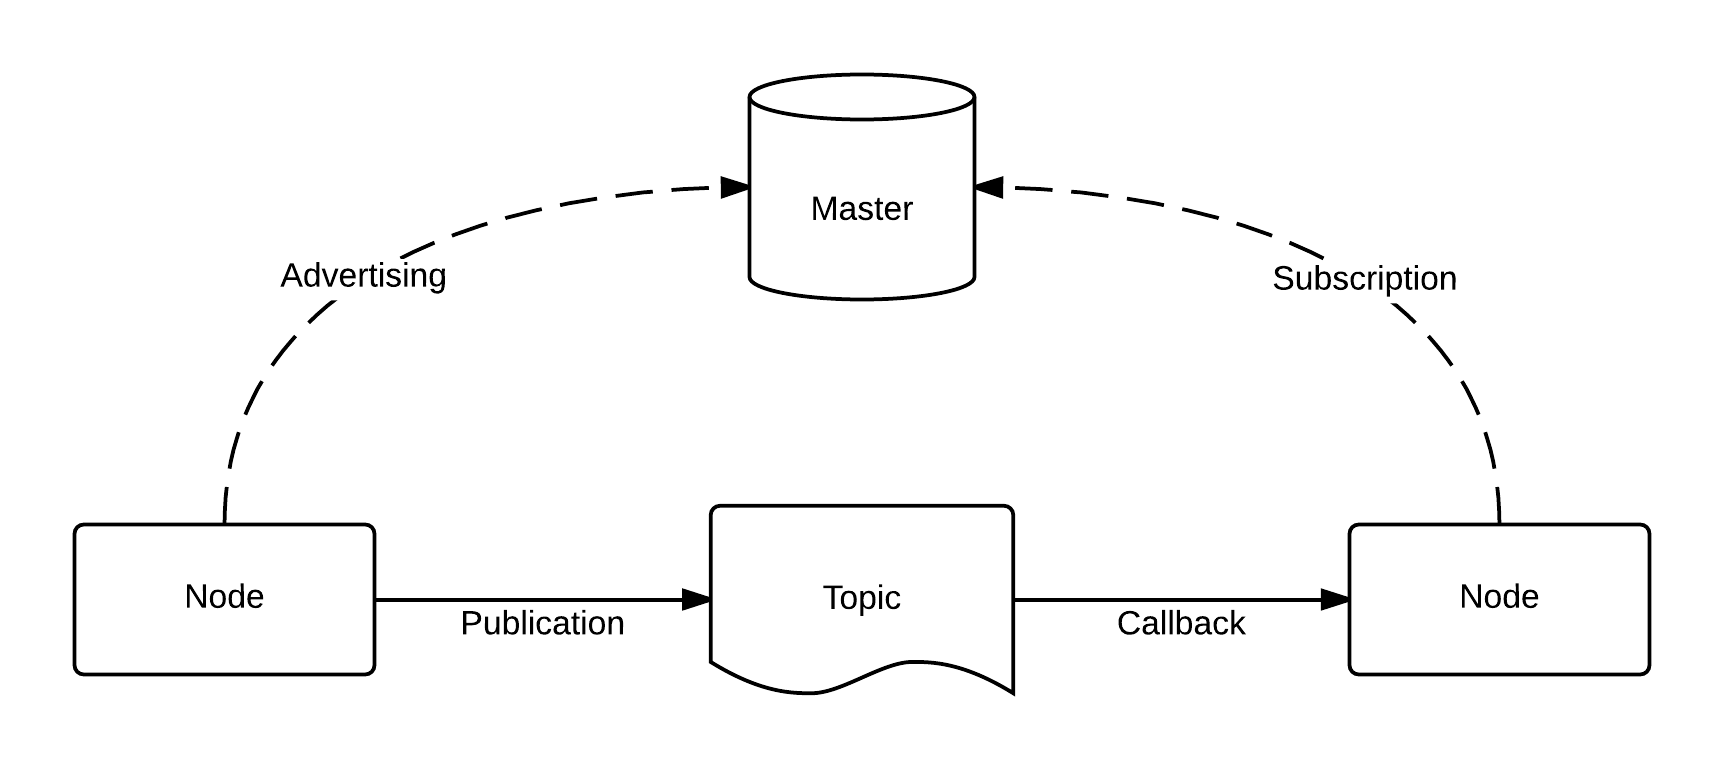
\includegraphics{Images/Chapter 1/ROS-master-node-topic.png}
    \caption{Visualization of Master-Node-Topic relationship}
    \label{fig:master-node-topic}
\end{figure}
\\
\newline
\textbf{Parameter server}\\
The parameter server is basically a component of the master, allowing certain configurations accessible via the network API to be shared publicly with all nodes. Although not an extremely high-performing it is nevertheless useful for the testing phase of the software. Parameters are named using the normal ROS naming convention. This means that ROS parameters have a hierarchy that matches the namespaces used for topics and nodes, \citet{rosparmserv}.

\chapter*{Theoretical background}
From now on some basic knowledge needed to comprehend the reasoning of this work's study object is described and explained. 
This section consists of:
\begin{itemize}
    \item \textbf{Chapter \ref{ch:ros}:} \nameref{ch:ros}
    \item \textbf{Chapter \ref{ch:robot}:} \nameref{ch:robot}
\end{itemize}

\chapter{ROS}
\label{ch:ros}
\section{Introduction}
In the field of robotics, platforms are of increasing importance. A platform is divided into a software platform and a hardware platform. There are a variety of features that make up robot software platforms, including low-level device control, SLAM (Simultaneous Localization and Mapping), navigation, manipulation, recognition of objects or people, sensing and package management, debugging and development tools, which are mostly used in the industrial sector where robot software platforms are currently primarily employed. Robot hardware platforms not only study platforms such as mobile robots, drones, and humanoids, but also commercial products. Hence, robot researchers from around the world are collaborating to discover a platform that is intuitive and open source. The most popular robot software platform is ROS, that means Robot Operating System. ROS, the Robot Operating System, is an open source framework to manage robots’ operations, tasks, motions, and other things. ROS is intended to serve as a software platform for those who build and use robots daily, but at the same time for people who are starting to use robots no long ago. This common platform allows newcomers to be increasingly inclined to read more and more and it is very easy to use. The design of the ROS platform allows the use of code and information shared by other programmers, which means you do not have to write all code in order to move the robots.
\newpage
\section{History of ROS}
“In May 2007, ROS was started by borrowing the early opensource robotic software frameworks including switchyard, which is developed by Dr. Morgan Quigley by the Stanford Artificial Intelligence Laboratory in support of the Stanford AI Robot STAIR (Stanford AI Robot) project.
Dr. Morgan Quigley is one of the founders and software development manager of Open Robotics (formerly the Open Source Robotics Foundation, OSRF), which is responsible for the development and management of ROS.
Switchyard is a program created for the development of artificial intelligence robots used in the AI lab’s projects at the time and it is the predecessor of ROS.
In addition, Dr. Brian Gerkey, the developer of the Player/Stage Project and 2D Stage simulator, later influence the growth of 3D simulator Gazebo, which was developed since 2000 and has had a major impact on ROS’s networking program. He is the co-founder of Open Robotics.
In November 2007, U.S. robot company Willow Garage succeeded the development of ROS. Willow Garage is a well-known company in the field of personal robots and service robots.” \cite{Quigley15}\\
Robots are computer-controlled electromechanical devices.
First dedicated robot programming languages arose in the 1970's.
There were robot-centric data types and some robot function libraries. They did not allow neither hardware abstractio, nor multi-robot interaction nor integrated simulation. There did not exist code reuse or standardization.
The efforts to build robot programming system continued through 80's, 90's and especially in the 2000's were there was a high push to standardize robot components, their interfaces and basic functions.\\
Hence, ROS as it is known today was initially developed in 2007 at the Standford Artificial Intelligence Laboratory. Since 2013 it is managed by OSRF and nowadays it is used by many robots, universities and companies, becoming the de facto standard for robot programming.
\begin{figure}[H]
    \centering
    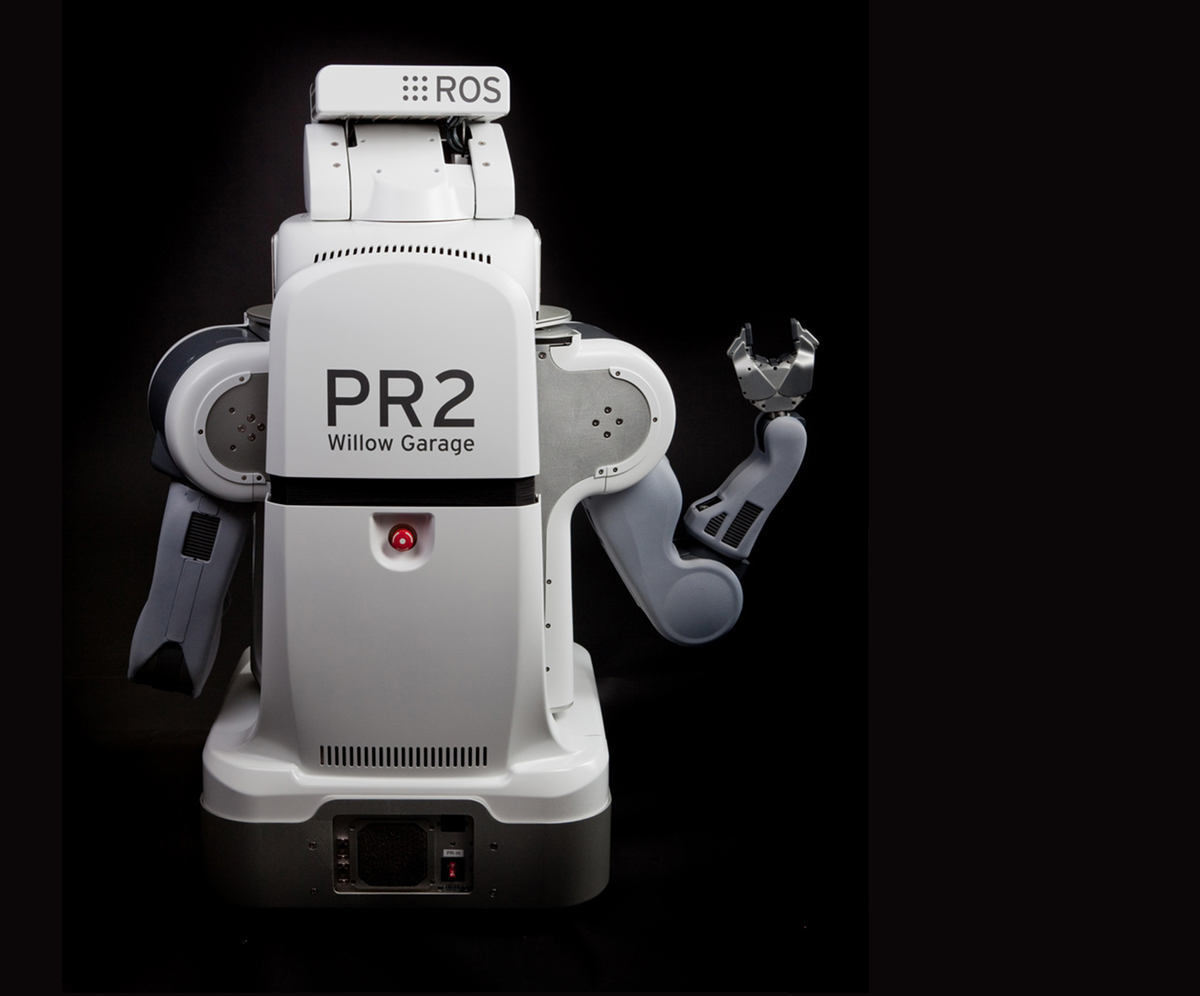
\includegraphics[scale=0.16]{Images/Chapter 1/PR2_Robot_Willow_Garage_6-1.jpeg}
    \caption{Willow Garage PR2 robot}
    \label{fig:PR2}
\end{figure}
\newpage
\section{Meta-Operating System}
ROS is an open source, meta operating framework for robots, hence it is nothing else than a middleware. \\
A middleware can be defined as a piece of software that gives an extra level of abstraction to the developer through a layer between the operating system and the applications.
It basically sits in the middle of software components and facilitates their interaction. \\
Its purpose is to provide an abstraction model for functions and at the same time provides the low-level implementation.
Every middleware must provide:
\begin{itemize}
    \item Portability: common programming model regardless the programming language and system architecture
    \item Complexity management: low-level aspects are managed by libraries and drivers inside the middleware itslef
    \item Reliability: middleware allows robot developer to discard low level details
    \item abstraction from sensors/actuators hardware;
    \item communication protocol for data transport
\end{itemize}
 As a result, they play an essential role in the development of complex applications that rely on a number of hardware and software tools.\\
 While they are still under active development, they are not yet capable of providing a complete set of functions for general purpose robots.
 
\begin{figure}[H]
    \centering
    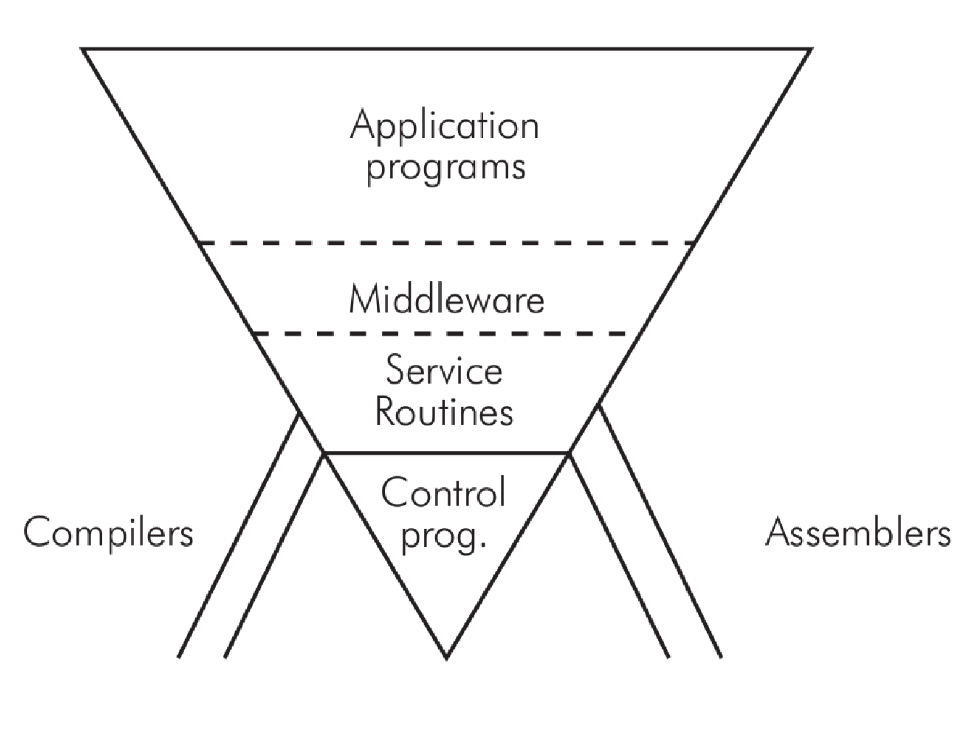
\includegraphics[scale=0.5]{Images/Chapter 1/middleware.png}
    \caption{Meta Operating System}
    \label{fig:metaoperating}
\end{figure}
 
 Several robotic middlewares have been proposed in the past years (OROCOS, ORCA, YARP, BRICS etc.) and eventually came ROS.
 
 \subsection{Phylosophy of ROS}
The following paragraphs describe some philosophical aspects of ROS:\\
\begin{itemize}
\item \textit{Peer to peer}: ROS systems consist of a small number of computer programs that are linked to one another and continuously exchange messages. These messages travel directly from one program to another. Although this makes the system more complex, the result is a system that balances better as the number of data increases.\\
\item \textit{Distributed}: Programs can be run on multiple computers and comunicate over the network.
\item \textit{Multilingual}: ROS chose a multilingual approach. ROS software modules can be written in any language for which a client library has been written. At the time of writing, client libraries exist for C++, Python, LISP, Java, JavaScript, MATLAB and others.\\
\item \textit{Thin}: the ROS conventions encourage contributors to create standalone libraries and then wrap those libraries, so that they can send and receive messages to and from other ROS modules. This extra layer is proposed to allow the reuse of software outside of ROS for other applications, and it greatly simplifies the creation of automated tests using standard continuous integration tools.\\
\item \textit{Free and open source}: the core of ROS is released under the permissive BSD license, which allows both commercial and non-commercial use. ROS foresees data exchange between modules using inter-process communication (IPC), which means that systems built using ROS can have fine-grained licensing of their various components.\\
\end{itemize}

\section{ROS Architecture}
ROS is based on a graph architecture where processing takes place in nodes, which communicate with each other by exchanging messages asynchronously through the use of topics to which they can subscribe to and/or on which they can publish, and synchronously with the calling of services, similar to RPCs.  Structurally, ROS is developed on 3 conceptual levels, File-system Level, Computational Level and Community Level, of which we are going to examine the constituent elements and their role in the architecture.
\subsection{File-system Level}
The Filesystem Level includes all resources used in ROS, in particular
\begin{itemize}
    \item Packages
    \item Metapackages
    \item Manifest
    \item Message types
    \item Service types
\end{itemize}
\begin{figure}
    \centering
    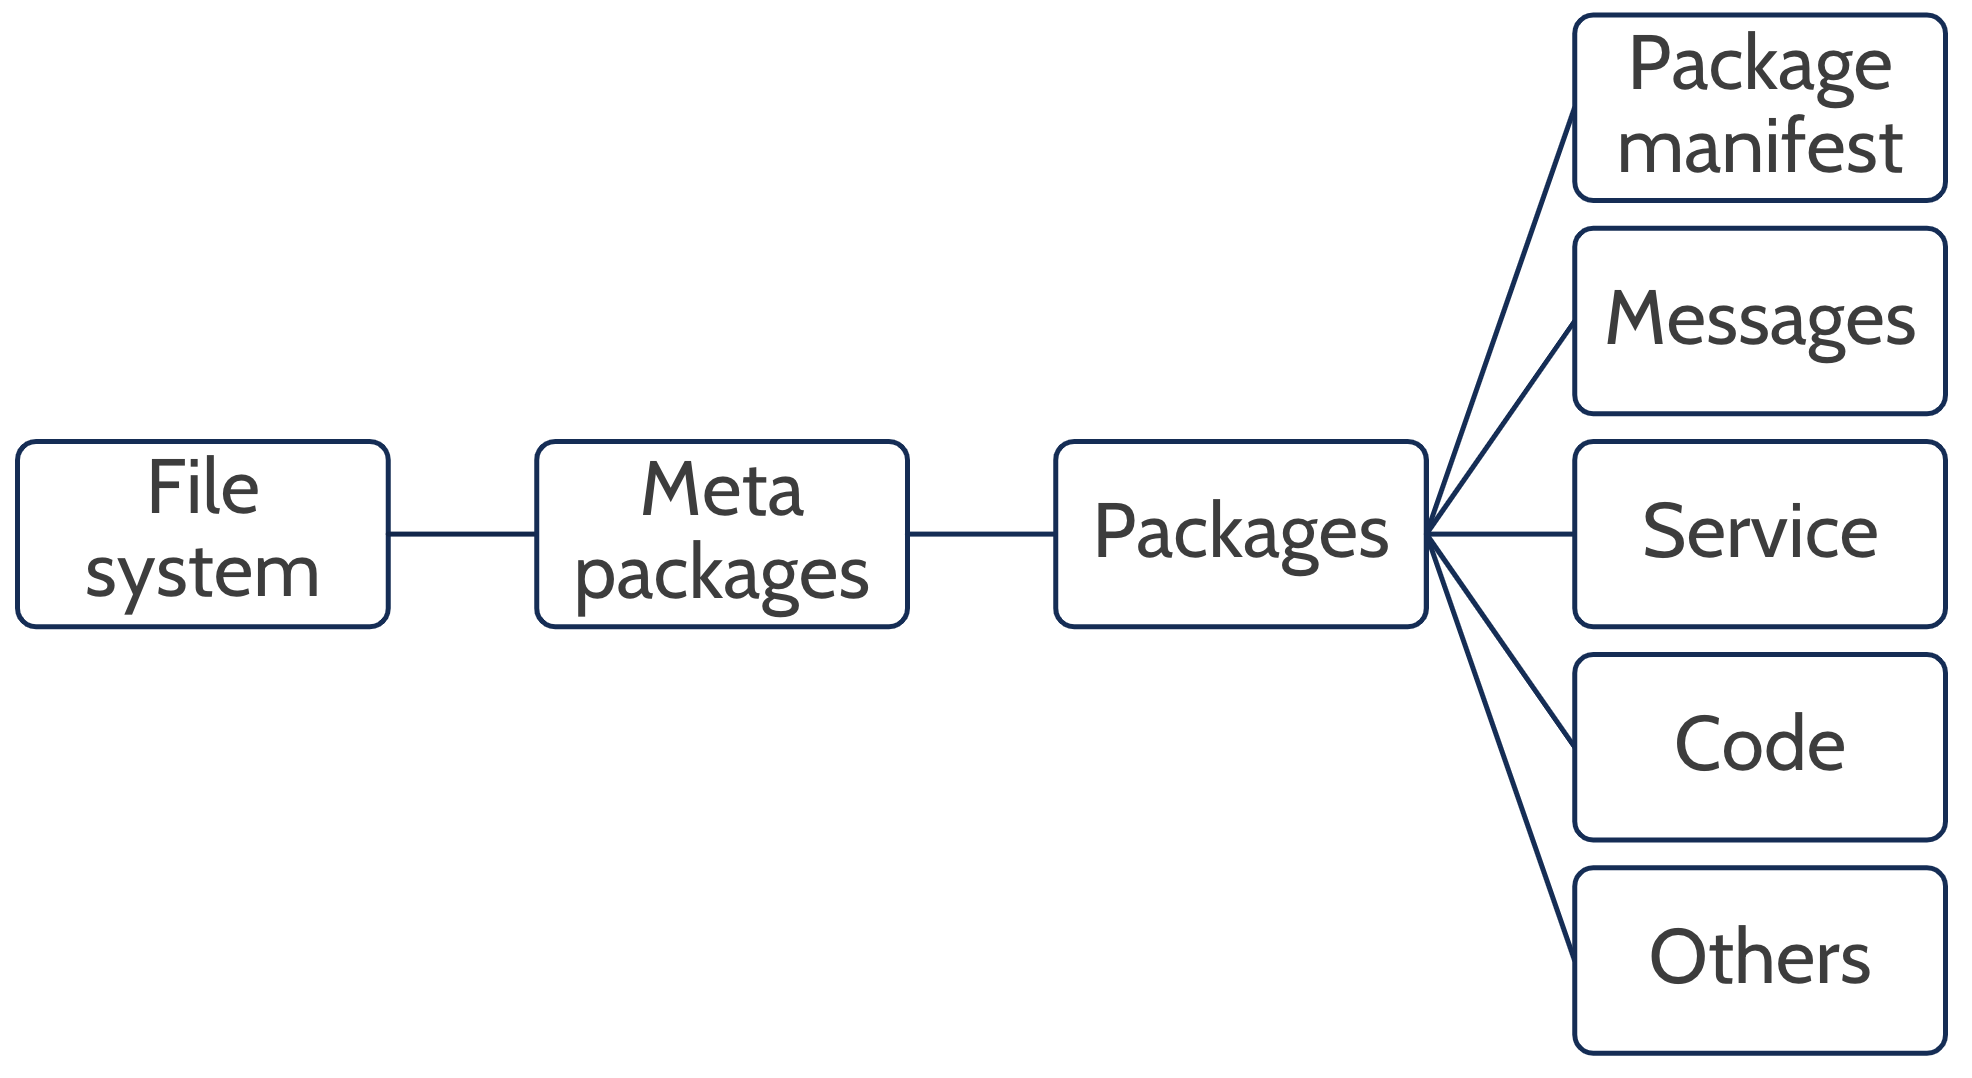
\includegraphics[scale=0.5]{Images/Chapter 1/Filesystem.png}
    \caption{File System level representation}
    \label{fig:Filesystem}
\end{figure}
\textbf{Packages}\\
Packages are the main structure for organising ROS  \citet{rospackages}. The processes, libraries, configuration files, datasets, and all the files used by the system at runtime are stored in these files. They are the structure that can be found within a ROS-based system. At the filesystem level, the package is represented by a directory. The structure within it includes some subfolders to manage the elements
In order to facilitate its development, in particular:
\begin{itemize}
    \item \textit{include/packagename}: C++ include headers (make sure to export in the CMakeLists.txt)
    \item \textit{msg}:Folder containing Message (msg) types
    \item \textit{src/packagename}: Source files, especially Python source that are exported to other packages.
    \item \textit{srv/}: Folder containing Service (srv) types
    \item \textit{scripts}: executable scripts
    \item \textit{CMakeLists.txt}: CMake build file
    \item \textit{package.xml}:XML file containing package structure 
    \item \textit{CHANGELOG.rst}: Many packages will define a changelog which can be automatically injected into binary packaging and into the wiki page for the package
\end{itemize}\\

\textbf{Metapackages}\\
Metapackages are specialised structures whose only task is to represent a group of packages that have common characteristics with each other. The metapackages that are created in the context of older versions of ROS and later updated may also result from the conversion of older stacks that perform similar functions in the context of older versions of ROS \citet{rosmetapackages}.\\
\newline
\textbf{Manifest}\\
A package manifest consists of an XML file named package.xml that must be included in the root folder of any catkin-compliant package. It contains information about the package, including its name, version number, authors, maintainers, and dependencies on other catkin packages. There is a strong similarity between this concept and the manifest.xml file used in the legacy rosbuild build system. System package dependencies are declared in package.xml \citet{rosmanifest}.\\
\newpage
There are a minimal set of tags that need to be nested within the <package> tag to make the package manifest complete.
\begin{itemize}
    \item \textit{<name>}: The name of the package
    \item \textit{<version>}: The version number of the package;
    \item \textit{<description>}: A description of the package contents;
    \item \textit{<maintainer>}: The name of the person(s) that is/are maintaining the package;
    \item \textit{<license}: The software license under which the code is released.
\end{itemize}
\textbf{Message types}\\
Message types define the structure of messages sent by ROS \citet{rosmsg}. Each file, with extension .msg, represents a different type of message. Within the file each line represents a message field. Each line, in turn, contains two columns: the first one for the data type of the field
(Int32/int (C++/Phyton), bool, string, time, etc.), the second for the name. It is possible to assign values to the fields within these le, in this case we speak of constants. Example of msg file (C++):

\textbf{Service types}\\
Service type are files that define the structure of request/response for ROS services \citet{rossrv}.
These are directly built upon the msg format to enable communication between nodes. They are stored in dedicated .srv files in the srv/ subdirectory of a package.
Example of srv file (C++):
\begin{lstlisting}[language=C++]
 bool add(beginner_tutorials::AddTwoInts::Request  &req,
             beginner_tutorials::AddTwoInts::Response &res)
    {
      res.sum = req.a + req.b;
      ROS_INFO("request: x=%ld, y=%ld", (long int)req.a, (long int)req.b);
      ROS_INFO("sending back response: [%ld]", (long int)res.sum);
     return true;
   }
\end{lstlisting}

\newpage

\subsection{ROS Computational Graph Level}
The Computation Graph is the peer-to-peer network of ROS processes that are processing data together. The basic Computation Graph concepts of ROS are nodes, Master, Parameter Server, messages, services, topics, and bags, all of which provide data to the Graph in different ways \citet{rosconcepts}.\\
\begin{figure}[H]
    \centering
    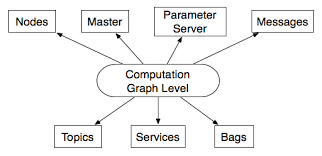
\includegraphics{Images/Chapter 1/computationgraph.png}
    \caption{Computation Graph}
    \label{fig:computationgraph}
\end{figure}
\textbf{Nodes}\\
A node is a process that performs computation. Nodes are combined together into a graph and communicate with one another using streaming topics, RPC services, and the Parameter Server \citet{rosnodes}. Following the concept of modularity of the system, each node will be related to only one specific functionality.\\ ROS in fact
discourages the creation of 'omnipotent' nodes that perform many functions in order to make the system more maintainable, reusable and clear.\\
The use of nodes in ROS provides several benefits to the overall system. There is additional fault tolerance as crashes are isolated to individual nodes. Code complexity is reduced in comparison to monolithic systems.\\
\newpage
\textbf{Topics}\\
Topics are buses identified by a proper and unique name that allow messages to be exchanged between nodes. They implement a mechanism
of publishing and subscribing: nodes can be publishers and/or subscribers if they are set up to send or receive messages. The division between
data producer and data user is clear and separated by anonymity policies
between the nodes. Each topic may have a maximum number of messages to be kept
in the queue in case they accumulate, those in excess are not added to the queue and lost \citet{rostopics}.\\
\newline
\textbf{Services}\\
Services are a two-way communication tool between nodes. It is a mechanism that extends that of messages with the possibility
not only to send commands to a specific node but also to remain in
listening and receiving a structured response from it. Each service is
first described in an .srv file where the parameters and type of service are indicated in addition to the name of the service.
of the service, as well as the parameters and the type of return data (see Service type).
Within the server node, the service is represented by a function
which takes as input two pointers to objects of the server class: one
one will include the function parameters (Request), the other will collect the return value.
will collect the return value \citet{rosservice}\\
\newline
\textbf{Messages}\\
The nodes in the graph communicate by exchanging messages. These
may be simple and of a primitive type (integer 
oat, string, char, etc.)
or arrays or even more complex, with structures similar to those seen in
C.\\
\newline
\textbf{Bags}\\
Bags represent the system by which ROS saves logs and keeps track of
all messages exchanged within a topic. The rosbag tool, once
associated with a topic, saves each message exchanged within a related file with the extension .bag. It is
very useful for storing data from the
sensors as it allows the developer to create a sort of "black box" of the robot.
black box" of the robot. ROS also provides a playback tool that allows the
visualise and playback the collected data via a graphical interface.\\
\newpage
\textbf{Master}\\
The master in ROS first takes care of registering new nodes within the
network, then managing the connection between the nodes in the graph, routing
messages and allowing access by one node to the services of another.
It is the heart of the software and can only be active one master at a time. It can be started via the roscore command or launched automatically
at the start of a node through the correct implementation of the file.
\begin{figure}[H]
    \centering
    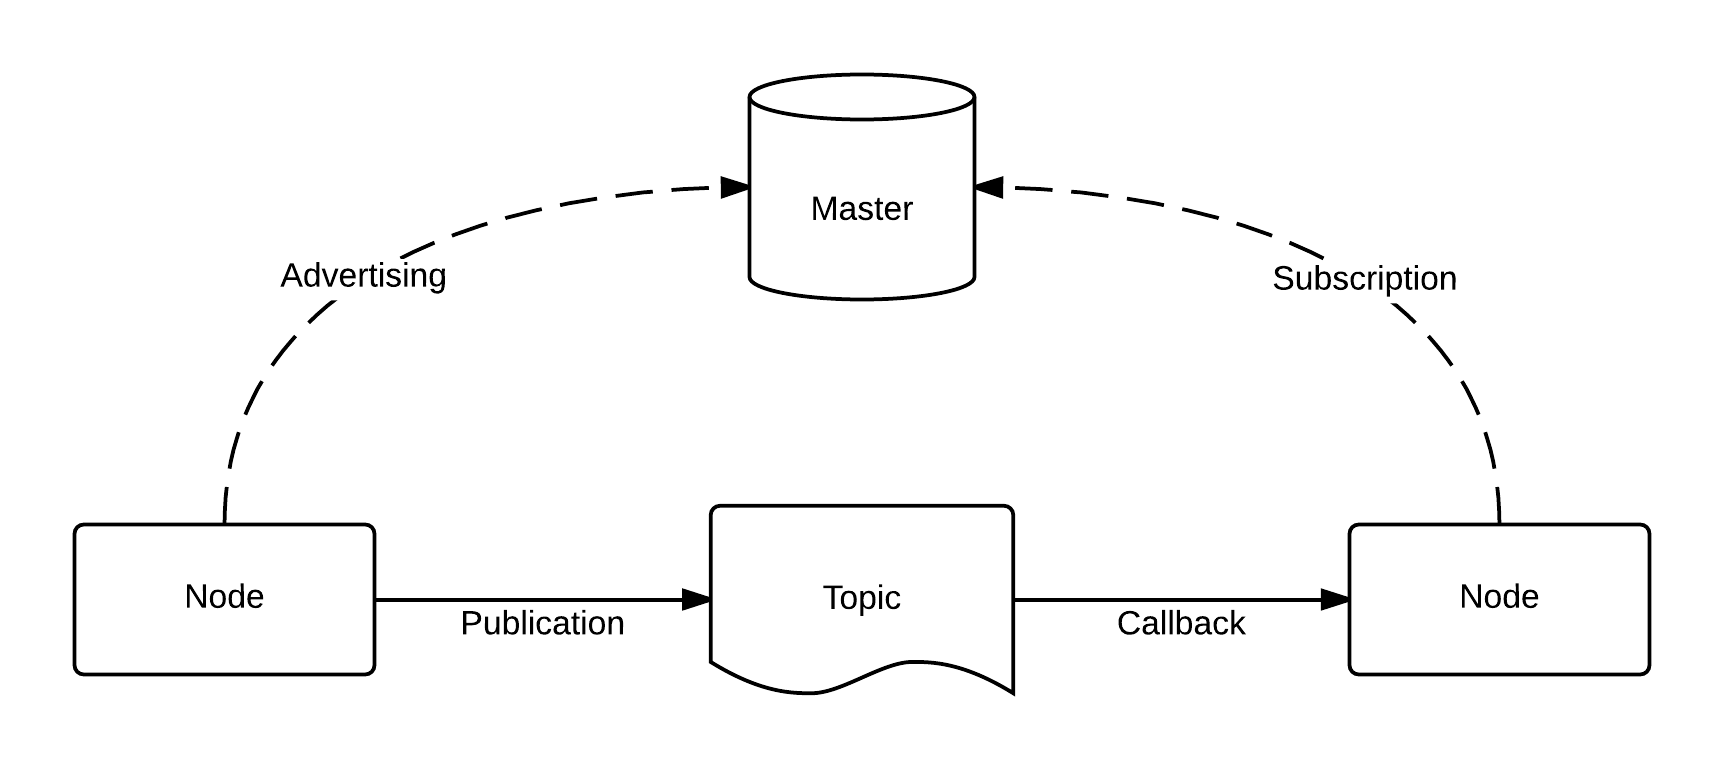
\includegraphics{Images/Chapter 1/ROS-master-node-topic.png}
    \caption{Visualization of Master-Node-Topic relationship}
    \label{fig:master-node-topic}
\end{figure}
\\
\newline
\textbf{Parameter server}\\
The parameter server is basically a component of the master, allowing certain configurations accessible via the network API to be shared publicly with all nodes. Although not an extremely high-performing it is nevertheless useful for the testing phase of the software. Parameters are named using the normal ROS naming convention. This means that ROS parameters have a hierarchy that matches the namespaces used for topics and nodes, \citet{rosparmserv}.

\chapter{Robot}
\label{ch:robot}
\section{Introduction}
\\
\\
\\
\begin{center}
    \textit{<<In the twenty-first century the \\
    robot will take the place which \\
    slave labor occupied in ancient \\ 
    civilization. There is no reason at \\ 
    all why most of this should not \\
    come to pass in less than a century, \\
    freeing mankind to pursue its \\
    higher aspirations.>>} \\ 
            \text{Nikola Tesla (1856 - 1943) }
\end{center}


\begin{center}
    \textit{<<Robots of the world! \\
    The power of
man has fallen!\\ A new world has
arisen:\\ the Rule of the Robots!
March!>>}\\
    \text{Rossum's Universal Robot (1920)}
\end{center}

Man has always spent his life working. Dangerous and degrading work has been the cause of death for many people for centuries. 
In this sense, there has always been a tendency to try to relieve man of the heaviest jobs by looking for machines or automatic systems to replace him.
In a sense, with the advent of the industrial revolution, we witnessed the first real process of robotizing in history.
On the other hand, with the evolution of discoveries in the medical field, the desire and curiosity arose in man to try to clone himself, artificially constructing his own like.
It is here that these two needs and tendencies come together in what we now call humanoid robots.
Indeed, humanoid robots are designed and built to replace humans in the most physical and repetitive tasks, in order to ensure greater well-being.

\newpage

\section{History of Robotics}
In recent years, the general public has become increasingly interested in robots and robotics research. New developments, e.g. robotic competitions, which "push beyond the boundaries of current technological
systems" (such as Defense Advanced Research Projects Agency (DARPA) in the
United States), especially in the area of robotics, have promised and delivered
fully integrated systems, \citet{robocomp}.\\
But the idea of creating intelligent, useful machines for humans has existed since the beginning of mankind.
In fact, ever since civilisation, one of the most unattainable desires and ambitions for mankind has been to create artifacts of his own image.\\
From a historical perspective, the first example that can be interpreted as such dates back to 3500 B.C., with the legend of the giant Talus, the slave forged by Hephaestus.
Continuing in time and reaching the Babylonians in 1400 B.C., we can observe the creation of the first automatic machine, the clepsydra water clock.
Continuing through the centuries, creations became more and more technologically advanced and jumping back to the 1500s, we encounter Leonardo da Vinci and his many inventions.
\begin{figure}[H]
    \centering
    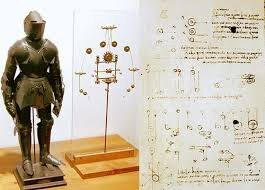
\includegraphics{Chapter 3/davinchiknight.jpeg}
    \caption{Leonardo da Vinci’s mechanical knight: sketches on the right, rebuilt
and showing its inner workings on the left.}
    \label{fig:my_label}
\end{figure}
The concept of the robot then gradually entered people's minds thanks to this long process, but it was only in the 20th century that it took on a real physical connotation.
\newline
The term 'robot' was introduced in 1920 by the play 'Rossum's Universal Robot', by Karel Čapek: it derives etymologically from the Slavic root word 'robota' meaning subordinate labor.
\begin{figure}[H]
    \centering
    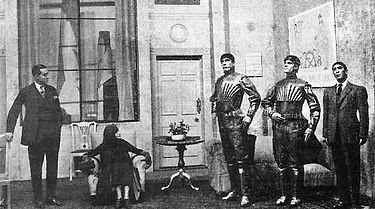
\includegraphics{Images/Chapter 3/rossumplay.jpg}
    \caption{A scene from Rossum's Universal Robot play, showing three robots}
    \label{fig:rossum}
\end{figure}
Later, during the middle of the century, the first research into the connection between human and machine intelligence was undertaken, marking the beginning of Artificial Intelligence (AI).
Between 1950 and 1980, Isaac Asimov wrote the so called "Three Laws of Robotics" in his book 'Runaround'. They are encoded in the "positronic brains" and are defined as follows, \citet{asimov}:
\begin{itemize}
\item A robot may not injure a human being or, through inaction, allow a human
being to come to harm.
\item A robot must obey the orders given to it by human beings, except where
such orders would conflict with the First Law.
\item A robot must protect its own existence as long as such protection does not
conflict with the First or Second Law.
\end{itemize}
Around those years, the first robots were created, they stemmed from the confluence of advances in two fields: numerically controlled machines for precision manufacturing and remote control to handle highly radioactive materials.
In fact, these two fields already featured modern applications of technologies such as mechanics, control, computational science and electronics.
The first robots were therefore master-slave arms, designed to reproduce the mechanics of the human arm but with rudimentary control and little perception.\\
During the second half of the century, the development of integrated circuits, digital computers and miniaturised components allowed terminal-controlled robots to be designed and developed.\\
In fact, in the 1980s, robotics was defined as the science that studies the connection between action and perception.In fact, action involves a locomotion apparatus that moves in the environment and a manipulation apparatus that performs actions, modifying its surroundings, thanks to special actuators and end-effectors.\\
Perception is then extracted from the sensors that provide information about the state of the robot (e.g. position and speed) and its surroundings (e.g. range and vision).
In the 1990s, research was further accelerated by the need to rely on robots to replace human presence in critical environments.\\
As we enter the new millennium, robots have undergone profound transformations both in their scope of use and in their shapes and sizes. 
\subsubsection{Humanoid Robots}
As reported in the article "Humanoid Robots:Historical Perspective, Overview and Scope", \citet{Siciliano2020}:\\
\\
"\textit{The long saga of humanoid robots in science fiction has influenced generations
of researchers, as well as the general public, and serves as evidence that people
are drawn to the idea of humanoid robots. Humans generally like to observe and
interact with one another. In their social behavior, people are highly attuned to
human characteristics, such as the sound of human voices and the appearance of
human faces and body motion. \\
Infants show preferences for these types of stimuli at
a young age, and adults appear to use specialized mental resources when interpreting these stimuli. By mimicking human characteristics, humanoid robots can engage
these same preferences and mental resources.\\
Throughout history, the human body and mind have inspired artists, engineers,
and scientists, using media as diverse as cave paintings, sculpture, mechanical toys,
photographs, and computer animation. \\
Humanoid robots serve as a powerful new
medium that enables the creation of artifacts that operate within the real world
and exhibit both human form and behavior. 
\\The field of humanoid robotics focuses
on the creation of robots that are directly inspired by human capabilities and/or
selectively imitate aspects of human form and behavior. Humanoids come in a
variety of shapes and sizes, from complete human-size legged robots to isolated
robotic heads with human-like sensing and expression.}"\\
Thus, humanoid robots were developed to be employed as multi purpose mechanical workers, and were designed to work alongside humans in daily tasks, being a support, living in the same environment and using the same tools.
It must also be considered that when the robot moves around in the work environment, there can be multiple risks for the worker; in this respect, a subfield of robotics, called cognitive robotics, has taken hold.
Indeed, robots can take advantage of the traditional communication methods used among humans to become more aware of their surroundings.
An even more ambitious aim is to interpret human gestures through vision (eye gaze, body language). On the other hand, this could put a human in a difficult relationship with the robot, modelled by the phenomenon called 'uncanny valley', a concept introduced in the 1970s by Masahiro Mori, a professor at the Tokyo Institute of Technology.
Masahiro in fact argues that:\\
"\textit{I have noticed that, in climbing toward the goal of making robots appear human, our affinity for them increases until we come to a valley, which I call the uncanny valley.}"
\begin{figure}[H]
    \centering
    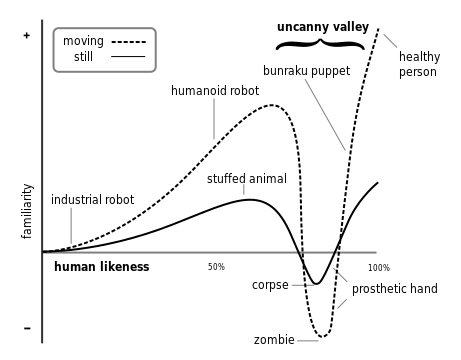
\includegraphics[scale=0.8]{Images/Chapter 3/Mori_Uncanny_Valley.png}
    \caption{Mori Uncanny Valley}
    \label{fig:mori_uncanny_valley}
\end{figure}
Mori better explains this concept with the example of the prosthetic hand:
\\
"\textit{One might say that the prosthetic hand has achieved a degree of resemblance to the human form, perhaps on a par with false teeth. However, when we realize the hand, which at first site looked real, is in fact artificial, we experience an eerie sensation. For example, we could be startled during a handshake by its limp boneless grip together with its texture and coldness. When this happens, we lose our sense of affinity, and the hand becomes uncanny.}"
\\
On the other hand, many scientists and researchers in the robotics community see humanoid robots as a possibility to better investigate human nature itself.
A part from the roles mentioned above, a humanoid robot could work as an avatar for telepresence, test ergonomics and serve for any other  roles that a human can do.
Even though in the past decades, humanoids have only been applied in research field, times seem to be mature to put these robots on field and let them cooperate with humans.
\section{Robee: Oversonic Robotics configuration}
In order to make physical sense of the results obtained within this project, it is important to define what technologies were used and what materials made up Robee's hardware.
\subsection{Hardware components and software architecture}
It is important to bear in mind that the Oversonic project has an architecture split between the
robot (also referred to as the edge) and the cloud, and these two components coexist in a
hybrid.
Describing the system from the cloud, the hardware component consists of a scalable node pool based on
the 2.35Ghz AMD EPYC 7452 processor that can achieve a boosted maximum frequency
of 3.35GHz with 32 GB RAM memory, running a Kubernetes instance on top of Linux
Ubuntu 18.04 (Bionic Beaver).
As far as the robot is concerned, all the computational power is provided by 2 Intel NUCs 8 including an Intel Core i5-8259U Processor (6M Cache, up to 3.80 GHz), 8 GB RAM and Integrated Graphics Intel Iris Plus 655.
The operating system which is mounted on is Linux Ubuntu 20.04 (Focal Fossa), and all the modules are running containers that on turn are managed by KubeEdge, a containers orchestration system built on Kubernetes.
\begin{figure}[H]
    \centering
    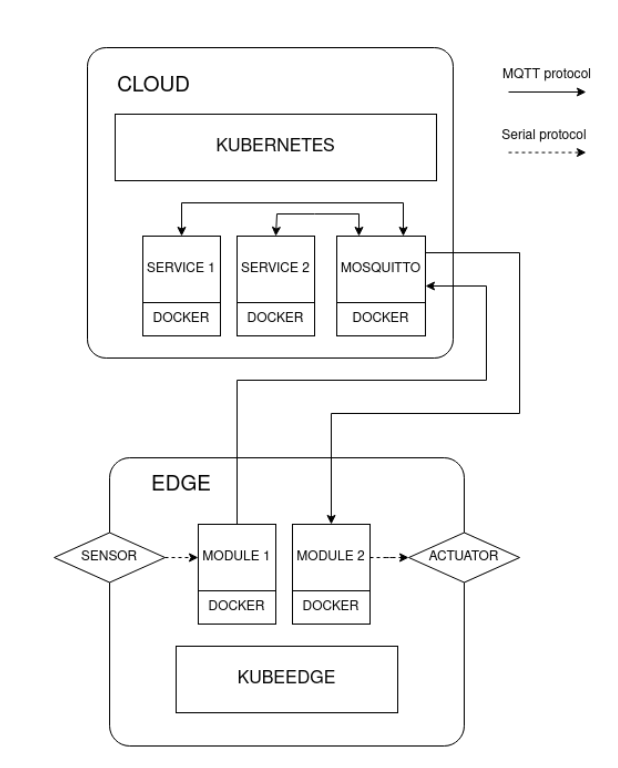
\includegraphics[scale=0.6]{Images/Chapter 3/oversonicarch.png}
    \caption{Oversonic Architecture}
    \label{fig:oversonicarch}
\end{figure}
\textbf{Internet of Things}\\
In the case of the Robee project, the architecture is therefore composed of various software modules that are containerised and must be able to communicate with each other.
The MQTT protocol is an optimal choice for this case.\\
From the official MQTT.org site: "\textit{MQTT is an OASIS standard messaging protocol for
the Internet of Things (IoT). It is designed as an extremely lightweight publish/subscribe
messaging transport that is ideal for connecting remote devices with a small code footprint and minimal network bandwidth. MQTT today is used in a wide variety of industries, such as automotive, manufacturing, telecommunications, oil and gas}", \citet{mqtt}.\\
MQTT therefore operates at the application layer of the OSI model, relying on TCP at the transport layer.
The MQTT protocol establishes two kinds of entities in the network: a message broker and a number of clients. The broker is nothing more than a server that receives all messages from all clients and then routes these messages to the relevant destination clients. A client is anything that can interact with the broker to exchange messages. The messages are routed to clients basing
on topics: every message is published over a specific topic, and only the clients subscribed
to it will receive the message.\\ A client, therefore, can be an IoT sensor or an application in a data centre that processes IoT data.
Each MQTT message has a command and a payload. The command defines the type of message:
\begin{itemize}
    \item CONNECT: initial message sent from client to broker, to instantiate a new connection
    \item DISCONNECT: final message sent from client to broker to end the connection
    \item PUBLISH: command to publish a message over a specified topic, it is sent from client to broker and then routed from broker to every client that appears to be subscribed to that topic
    \item SUBSCRIBE: message sent from client to broker in order to request a subscription to a specified topic
\end{itemize}
All MQTT libraries provide simple ways to handle such messages directly and can automatically populate certain required fields, such as 'message' and 'client Id'.
\begin{figure}[H]
    \centering
    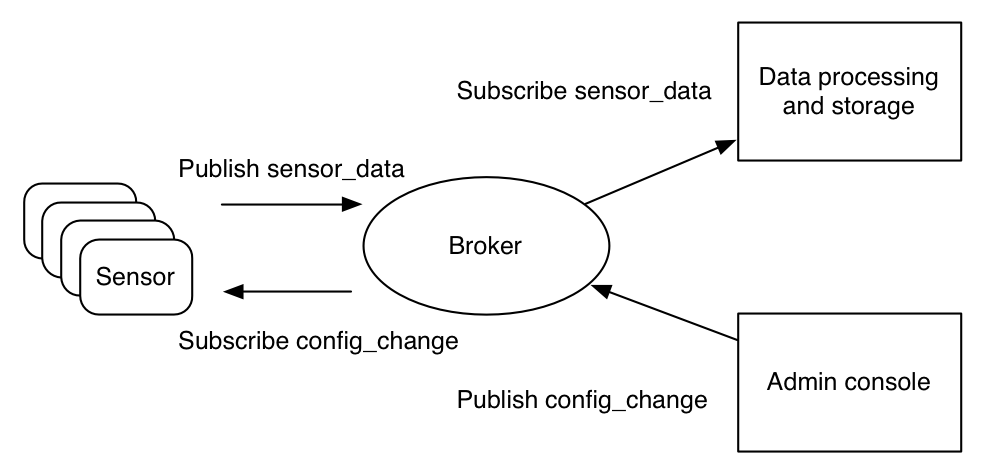
\includegraphics[scale = 0.8]{Images/Chapter 3/mqtt.png}
    \caption{The MQTT publish and subscribe model for IoT sensors}
    \label{fig:mqtt}
\end{figure}
\subsection{Robots Configurations}
The robots covered by the work in this thesis are mainly three 
\begin{itemize}
    \item R007 is a small autonomous mobile robot used by Oversonic as a prototype in the testing phase and features skid steering kinematics. In fact, it has two belts with two torque motors. The system is based on an Intel NUC and peripherals: two or four lidar sensors, a tracking camera and a depth camera mounted on the top base. The use of this AGV (autonomous guided vehicle) is mainly conceived in conjunction with its larger 'brother' Robee or in industrial logistics environments.
    \begin{figure}[H]
        \centering
        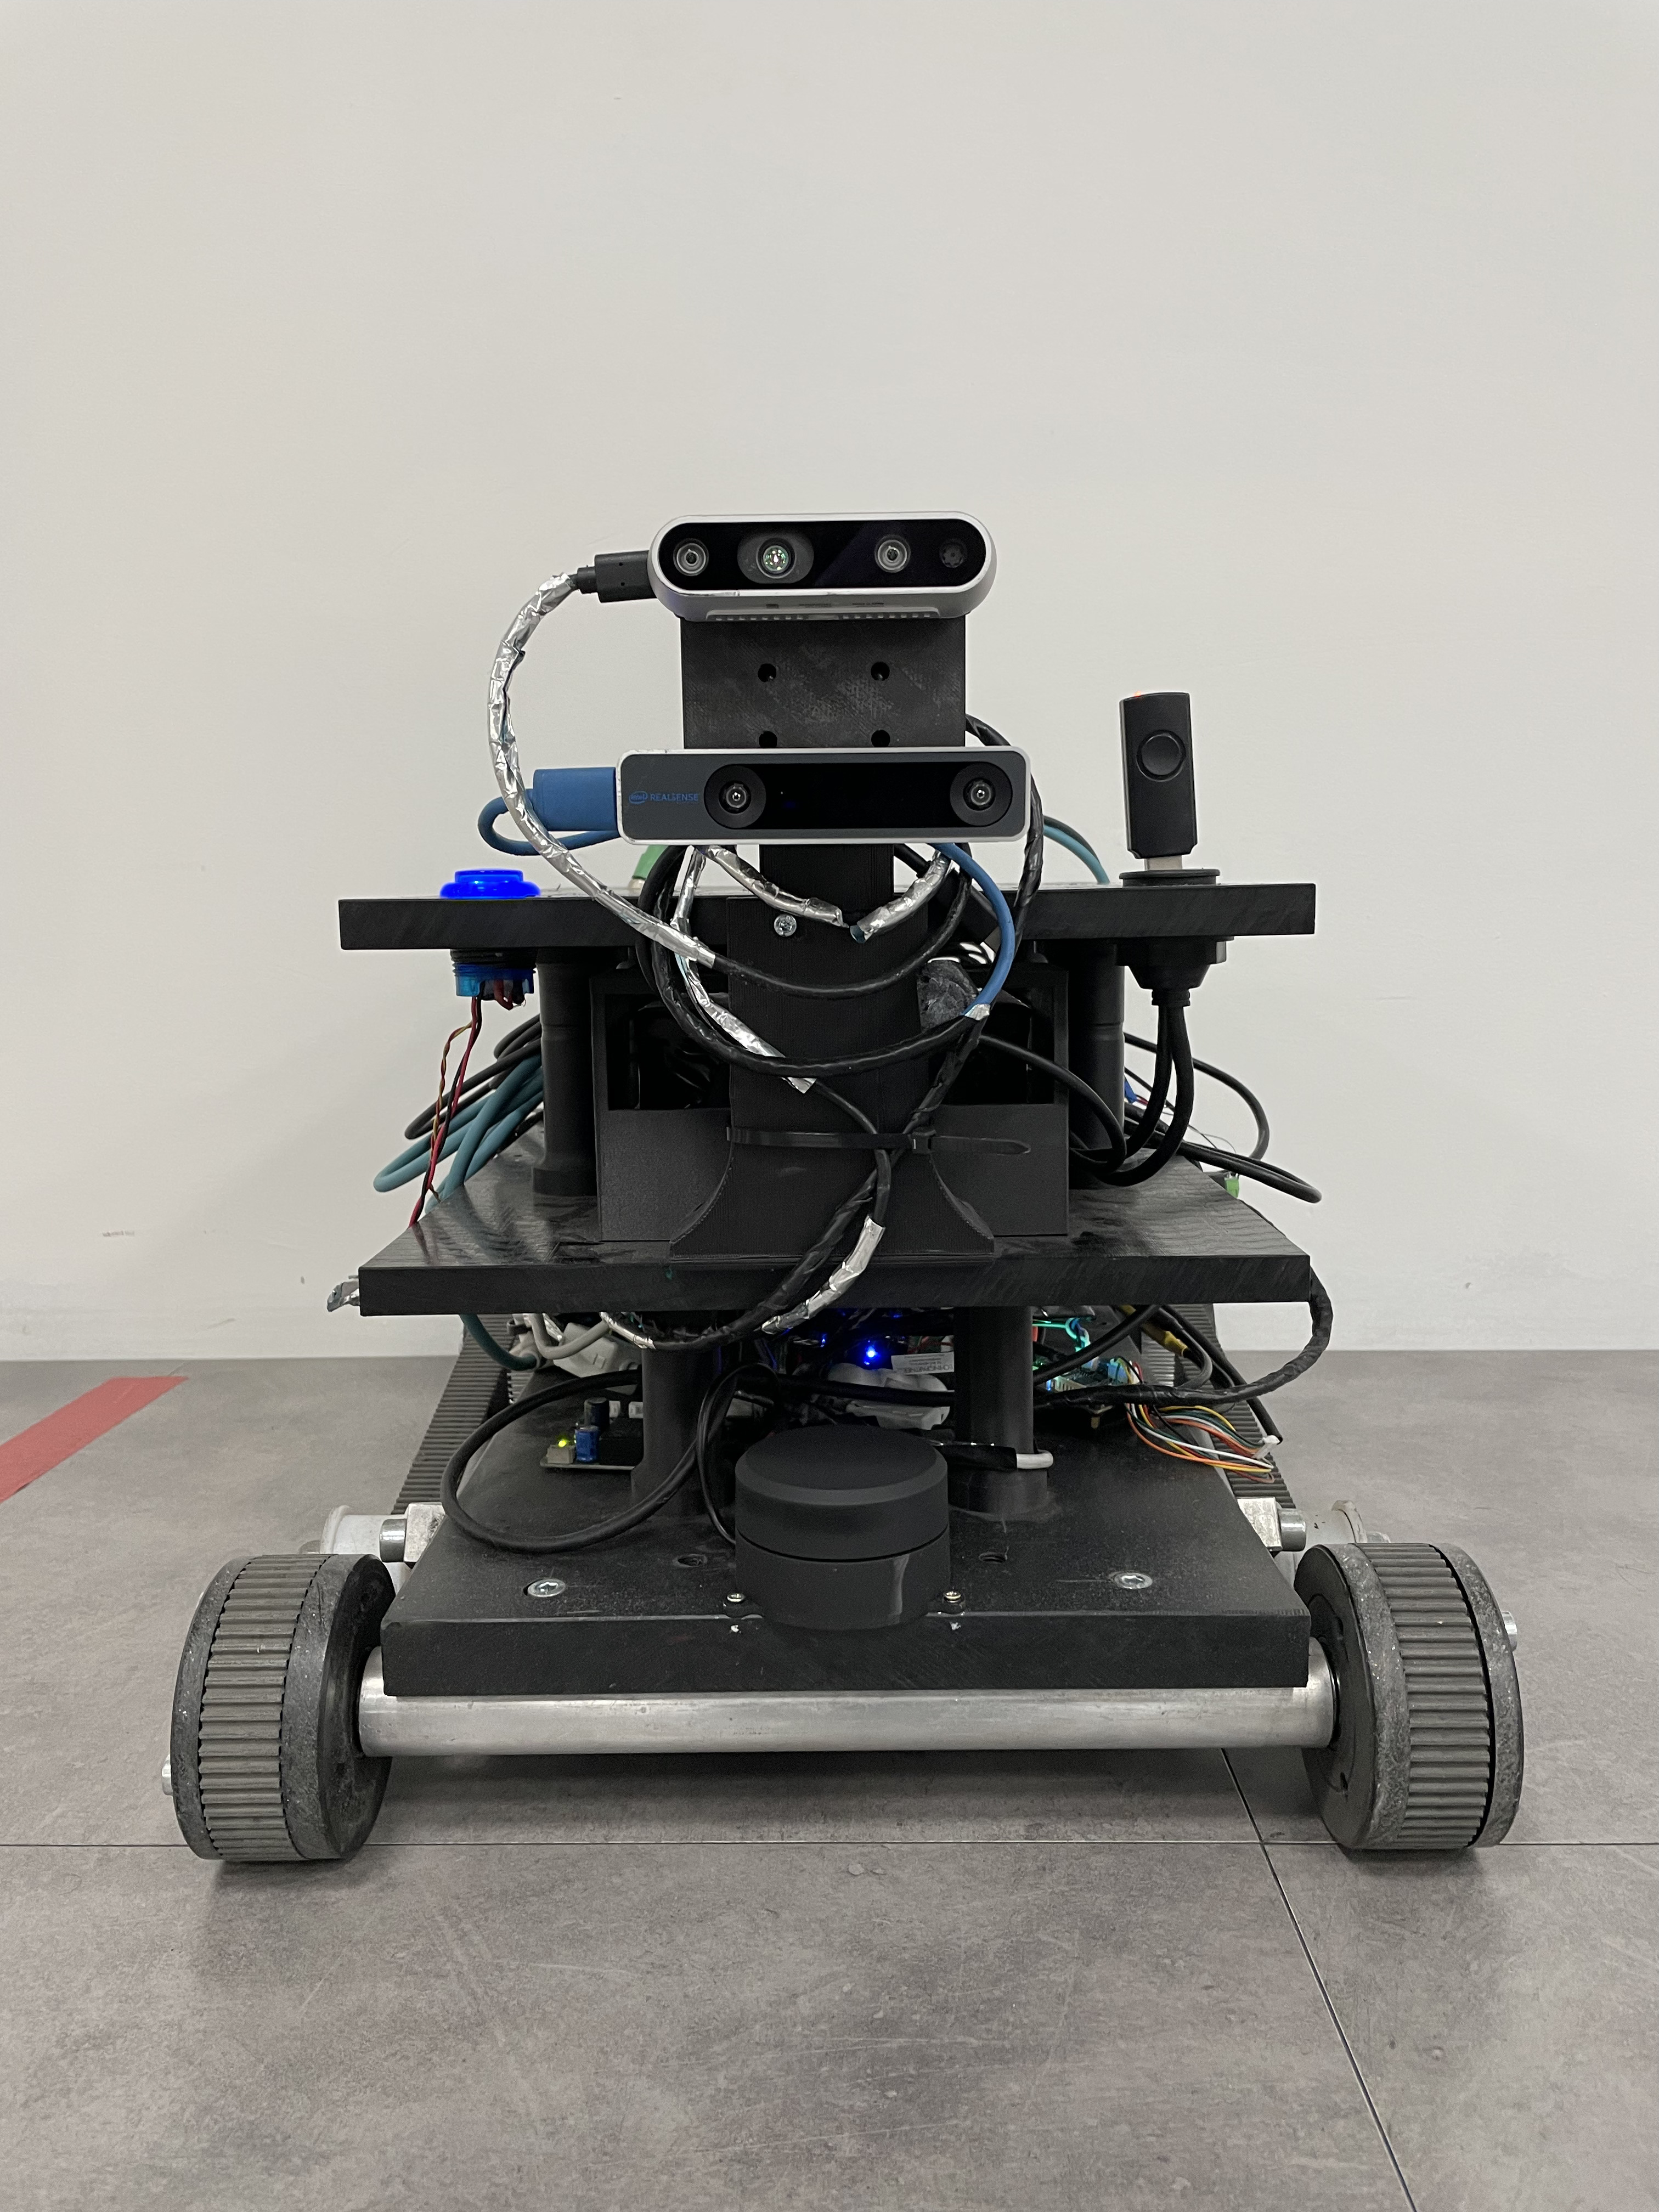
\includegraphics[scale=0.05]{Images/Chapter 3/r007.jpg}
        \caption{R007}
        \label{fig:r007}
    \end{figure}
    \item R012 is Oversonic's humanoid robot, now in its fourth evolution from the initial prototype and featuring a differential drive base. The system is divided into two parts, a lower body and an upper body, each featuring an NUC terminal and several sensors, but in this analysis we will focus exclusively on the lower part. 
    The lower body in fact contains within it the two torque motors, which move two wheels actively. For the robot's stability, two passive caster wheels have been added to the front and rear of the base. Two Lidar sensors are then mounted on the base and going up about halfway up the torso are a tracking and depth camera. 
    \begin{figure}[H]
        \centering
        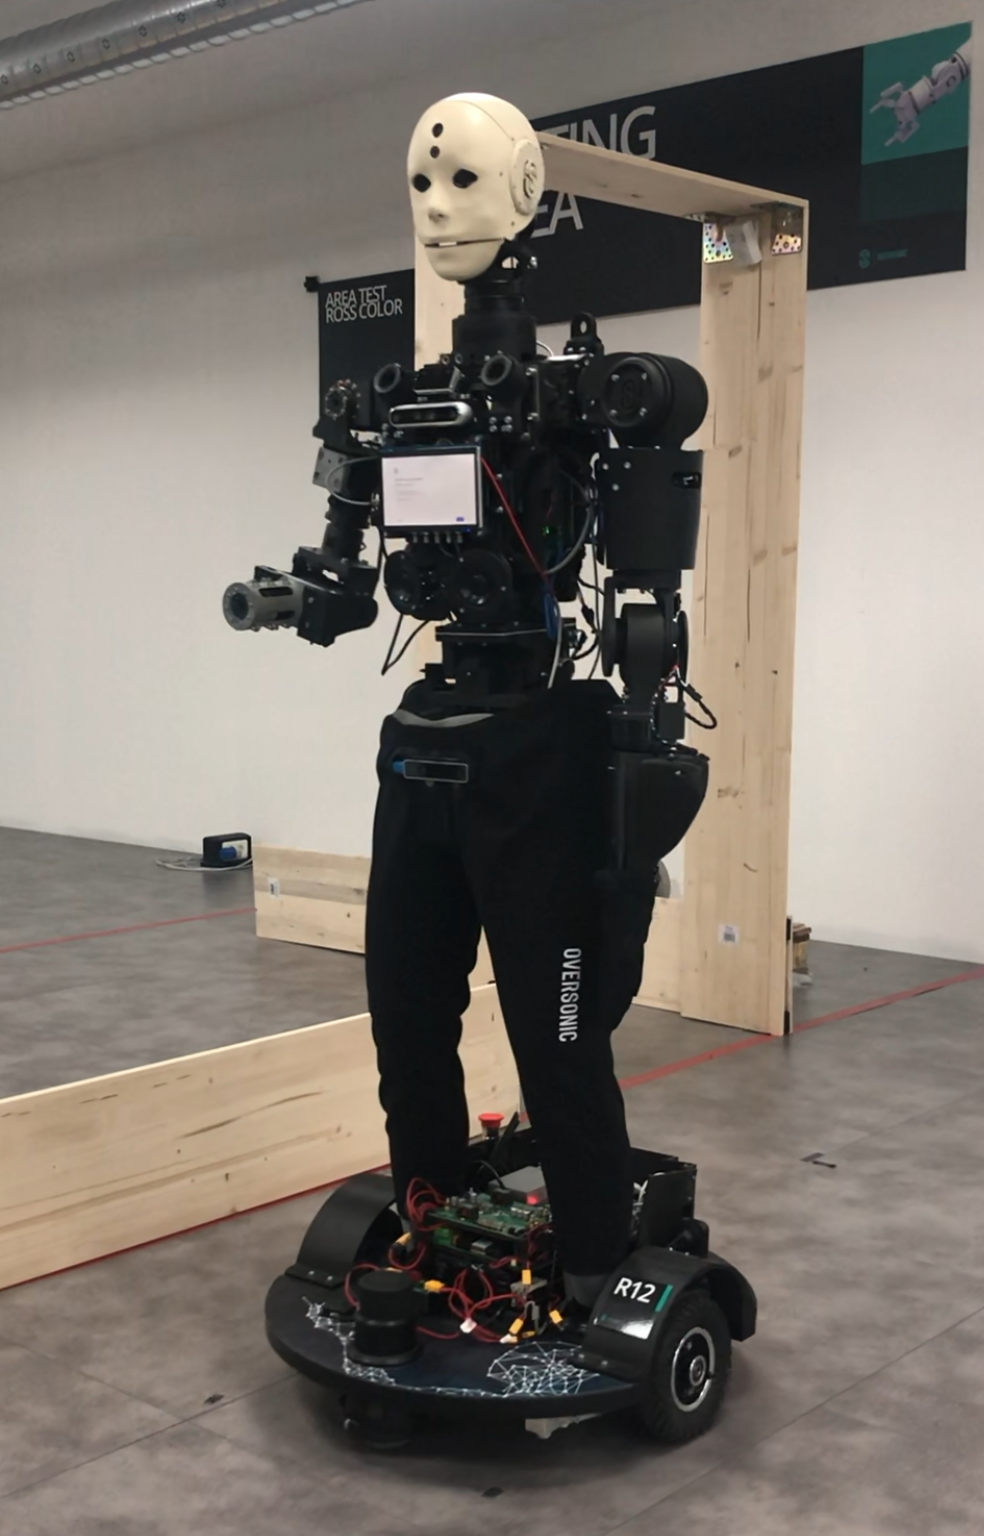
\includegraphics[scale=0.15]{Images/Chapter 3/r012.PNG}
        \caption{Robee R012}
        \label{fig:r012}
    \end{figure}
    \item N002 is a robot used for the testing phase of Robee's lower body. It has a similar purpose of use to R007.
    It has a differential drive base with two torque motor actuators, like R012 but with a physical arrangement of peripheral sensors but only one NUC.
    \begin{figure}[H]
        \centering
        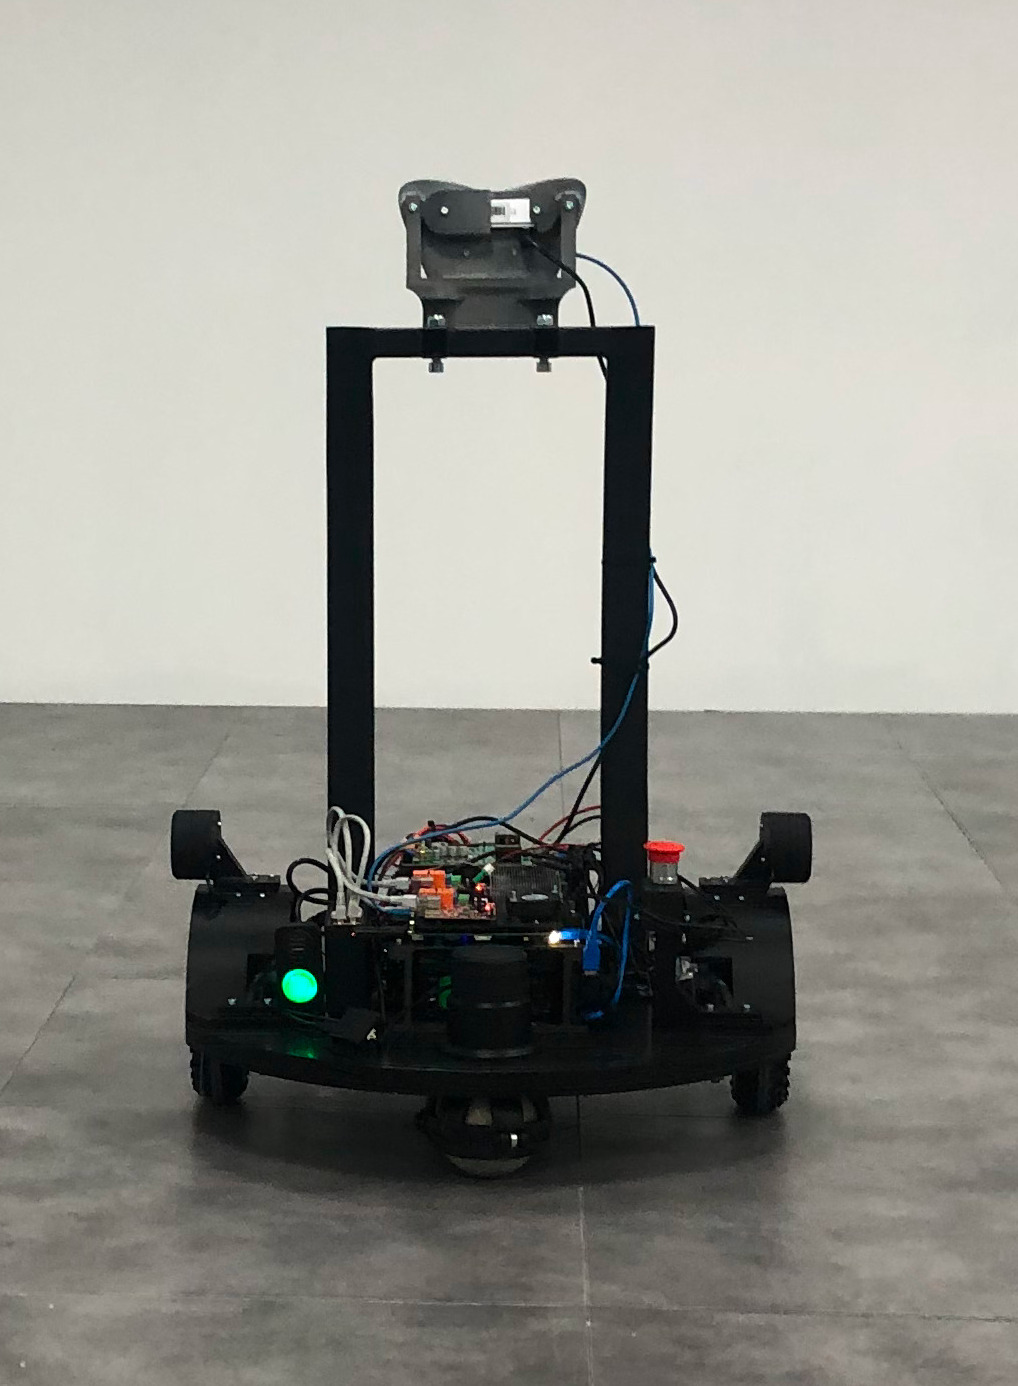
\includegraphics[scale=0.15]{Images/Chapter 3/n002.jpg}
        \caption{N002}
        \label{fig:N002}
    \end{figure}
\end{itemize}
The main features of the skid steering and differential drive kinematics will be listed below.
\textbf{Skid Steering}

Skid Steering is a particular kinematics configuration featuring two tracks. It is composed of two tracks on its basic configuration, left and right, and the control variables are indeed left and right speed.
Another configuration entails a 4 wheels set up featuring a low wheelbase configurations so that they can be deemed as two tracks.
When rotating the central point does not move as the track is sliding on the ground. It is clear that this drive needs proper calibration and slippage modeling in order to be reliable.
Some assumptions are needed for this kinematics model: the first, mass is placed in center of the fictitious medium, the second, all the wheels on the same side have the same speed.
While in motion, this kind of drive presents multiple ICR and all of them share the same $\omega_{z}$.
\begin{equation}
\begin{bmatrix}
    v_{x}\\
    v_{y}\\
    \omega_{z}
\end{bmatrix}
= J_{\omega} \begin{bmatrix}
\omega_{l}r\\
\omega_{r}r
\end{bmatrix}\end{equation}

 The wheels are turning and sliding simultaneously, resulting in two fictitious instantaneous centers of rotation: $ICR_{left}$ and $ICR_{right}$.
 Under proper assumptions, skid-steering can be simplified to a differential drive kinematics.
\begin{figure}[H]
    \centering
    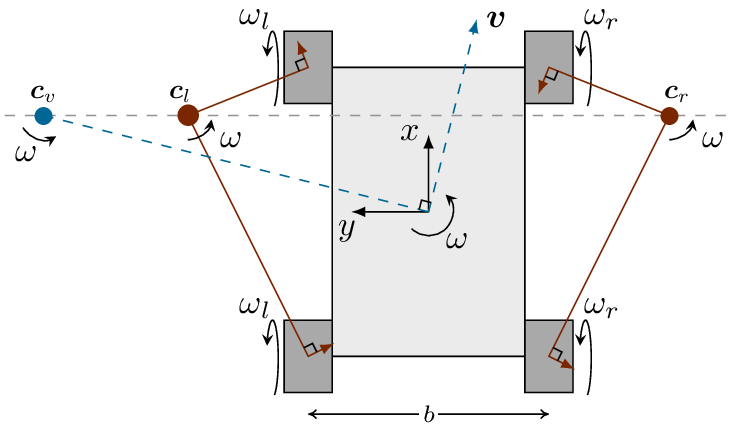
\includegraphics[scale=0.40]{Images/Chapter 3/skidsteer2.png}
    \caption{Skid Steering Kinematics}
    \label{fig:skidsteer}
\end{figure}
 Under proper assumptions, skid-steering can be simplified to a differential drive kinematics.
 
\textbf{Differential Drive}

Differential drive configuration present the following construction:
\begin{itemize}
    \item two wheels working on the same axis
    \item two independent motors, one for each wheel
    \item one or two passive caster wheels
\end{itemize}

Control input in this case are the linear and the angular velocity of the robot, \textit{v} and {\textomega}.
Wheels move around an Istantaneous Centre of Rotation on a circular path with istantaneous radius R and angular velocity \textomega.

\begin{equation}
    \begin{bmatrix}
    x' \\
    y' \\
    \theta \\
    \end{bmatrix} = \begin{bmatrix}
    \cos{\omega \delta t} & -\sin{\omega \delta t} & 0 \\
    \sin{\omega \delta t} & \cos{\omega \delta t} & 0 \\
    0 & 0 & 1
    \end{bmatrix}\begin{bmatrix}
    x - ICR_{x} \\
    y - ICR_{y} \\ 
    \theta'    \end{bmatrix} + \begin{bmatrix}
    ICR_{x} \\
    ICR_{y} \\
    \omega \delta t
    \end{bmatrix}
\end{equation}

It is therefore possible to reconstruct robot pose from direct kinematics:

\begin{equation}
    x(t) = \frac{1}{2}(\int_{0}^{t} (V_{R}(t') + V_{L}(t')) \cos{\theta(t')} \,dt')
\end{equation}

\begin{equation}
    y(t) = \frac{1}{2}(\int_{0}^{t} (V_{R}(t') + V_{L}(t')) \sin{\theta(t')} \,dt')
\end{equation}

\begin{equation}
    \theta = \frac{1}{b}(\int_{0}^{t} (V_{R}(t') - V_{L}(t')) \,dt')
\end{equation}


where $V_{R}$ and $V_{L}$ are defined as follows:
\begin{equation}
    V_{R} = \omega (R + \frac{b}{2}) 
\end{equation}

\begin{equation}
        V_{L} = \omega (R - \frac{b}{2})
\end{equation}

and as a consequence the following is derived:
\begin{equation}
    V = \frac{V_{R} + V_{L}}{2}
\end{equation}
\begin{equation}
    \omega = \frac{V_{R} - V_{L}}{2}
\end{equation}

It becomes clear that we can compute robot odometry by integrating the so-called control variables and knowing the parameters of the wheels, namely the direct kinematics.
On the contrary, we can derive control variables from a desired pose or velocity.


\begin{figure}[H]
    \centering
    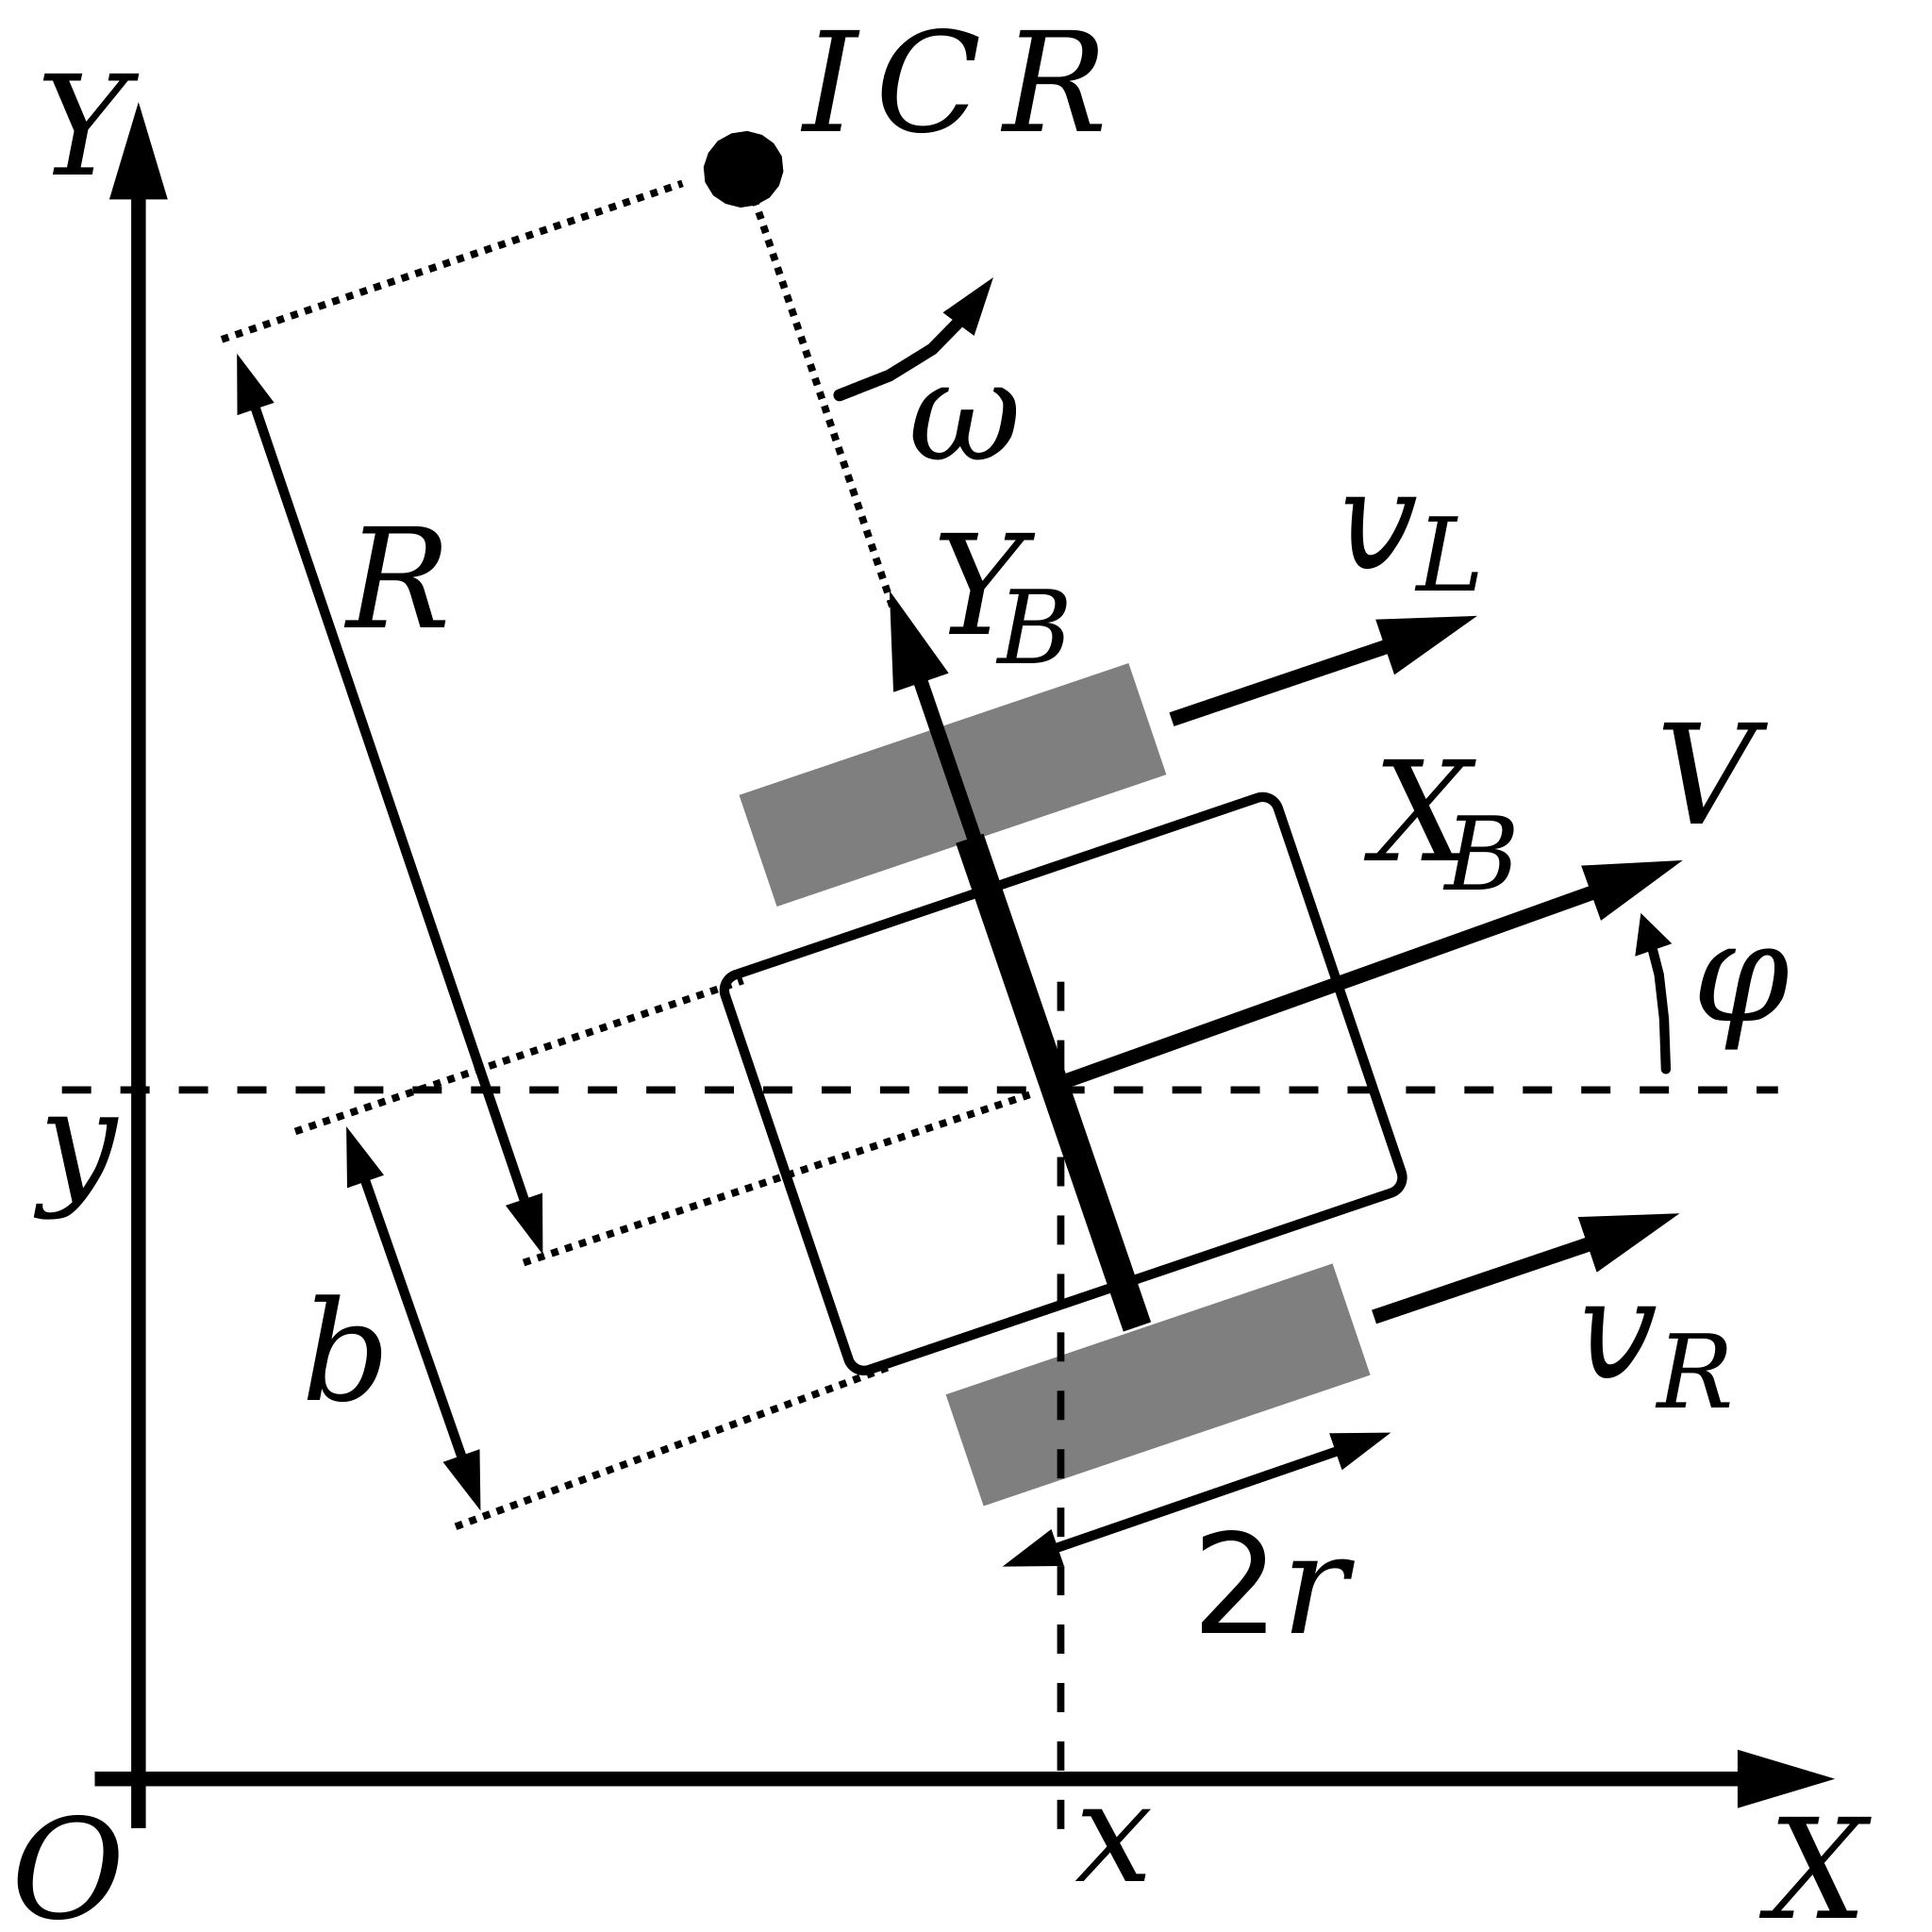
\includegraphics[scale=0.10]{Images/Chapter 3/diffdrive.png}
    \caption{Differential Drive Kinematics}
    \label{fig:diffdrive}
\end{figure}

It is interesting to mention three borderline cases for this kind of drive:
\begin{itemize}
    \item $V_{L}$ = $V_{R}$: forward linear motion is straight
    \item $V_{L}$ = - $V_{R}$: rotation in place
    \item $V_{L}$ = 0 or $V_{R}$ = 0: respectively, rotation about left and right wheel
\end{itemize}
\subsection{Sensors}
In order for a robot to perceive the world around it and to complete tasks autonomously, sensors are required. We distinguish between proprioceptive (internal state of the robot) and exteroceptive (state of the external environment) sensors. In this section, we focus on the exteroceptive sensors that have been used in Robee, providing a brief overview of their functioning.

\textbf{D400 Intel Depth Camera}

Depth cameras are a type of sensor widely used in robotic applications. They normally consist of two parts: a traditional digital camera, which captures RGB data, and a projector, which captures depth data.The depth system can work in several ways, for example by projecting a grid of light structured in a non-visible spectrum into a scene and then analysing the distortion created in this pattern to determine the distance and/or shape of any object placed in front, \citet{JONASSON2021112691}.
In our application, the main reason for using the d455 camera in Robee's lower body is ????distance measurement?????.
Traditional digital cameras shoot out an image as a grid of pixels in two dimensions. Each pixel is then associated with three values ranging from 0 to 255, which define the red, green and blue components, so black, for example, is (0,0,0) and a pure bright red would be (255,0,0). . This type of representation is called an RGB image. Thus, each image is composed of three channels each storing the values pertaining to each colour component.
\begin{figure}[H]
    \centering
    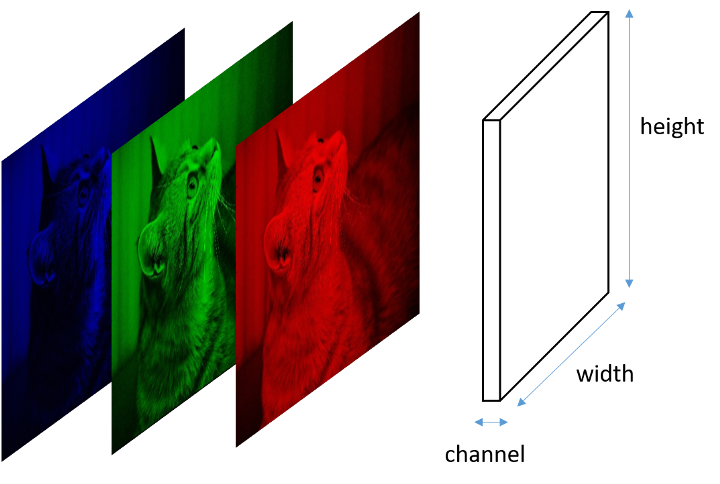
\includegraphics[scale=0.25]{Images/Chapter 3/rgb.jpeg}
    \caption{Channel decomposition}
    \label{fig:rgb}
\end{figure}
In the case of a depth camera, on the other hand, the pixels have different numerical values associated with them, where the number represents the distance of the corresponding pixel from the camera, thus the depth.
Thus, by unifying this representation we will have a colour map where cooler colours represent closer obstacles, and warmer colours represent more distant obstacles, in depth.

\begin{figure}[H]
    \centering
    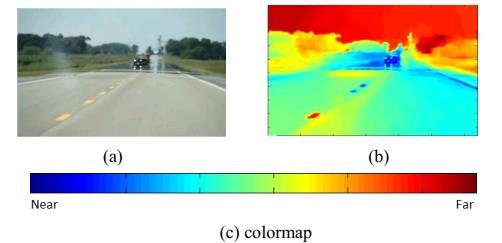
\includegraphics[scale=0.6]{Images/Chapter 3/depthmap.png}
    \caption{Depth-map representation}
    \label{fig:depthmap}
\end{figure}

\begin{figure}[H]
    \centering
    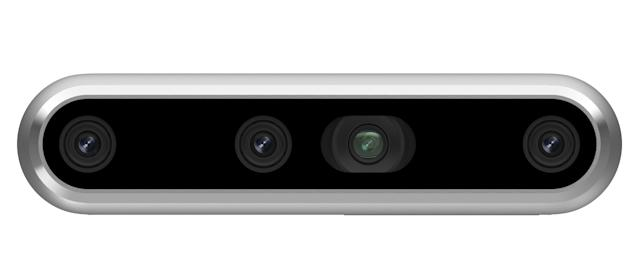
\includegraphics[scale = 0.5]{Images/Chapter 3/inteld455.jpeg}
    \caption{D455 Intel Tracking Camera }
    \label{fig:d455}
\end{figure}

Therefore, there are two types of three-dimensional image formats, the first being RGB-D and the second being pointcloud.
The first has already been introduced above, and we recall that for each pixel, identified by the coordinates (x,y), four properties (R,G,B,depth) are associated.
The substantial difference between the point cloud and RGB-D data is that in the pointcloud, the coordinates (x,y) represent the real world value instead of integer values. When viewing the two types of data, in fact, the former is presented in a sparse structure, while the latter is based on grid-aligned images. 
A practical application of point cloud will be provided in chapter \ref{ch:pcl}
\begin{figure}[H]
    \centering
    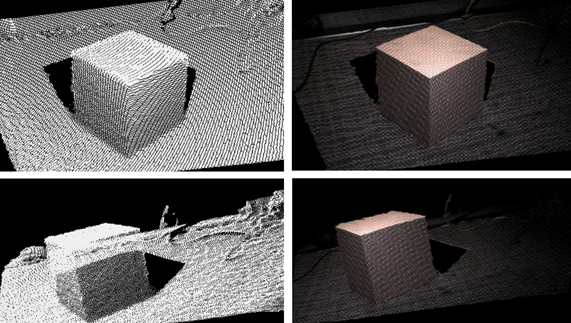
\includegraphics[scale=0.4]{Images/Chapter 3/pointcloudsample.png}
    \caption{Point Cloud sample}
    \label{fig:pointcloudsample}
\end{figure}
Thus, the point cloud can be constructed from RGB-D format images. In fact, by knowing an RGB-D dataset and the camera's intrensic values through a process called camera calibration. 
Since pointclouds are sets of disordered vectors, it is common for researchers to change the structure of the pointcloud data into 3D voxel grids.
The voxel grid geometry is in fact a grid of values in three dimensions, organised in layers of rows and columns.
The reason for this conversion also comes from the fact that one often then has to deal with deep learning models that expect highly regular input data formats.
\begin{figure}[H]
    \centering
    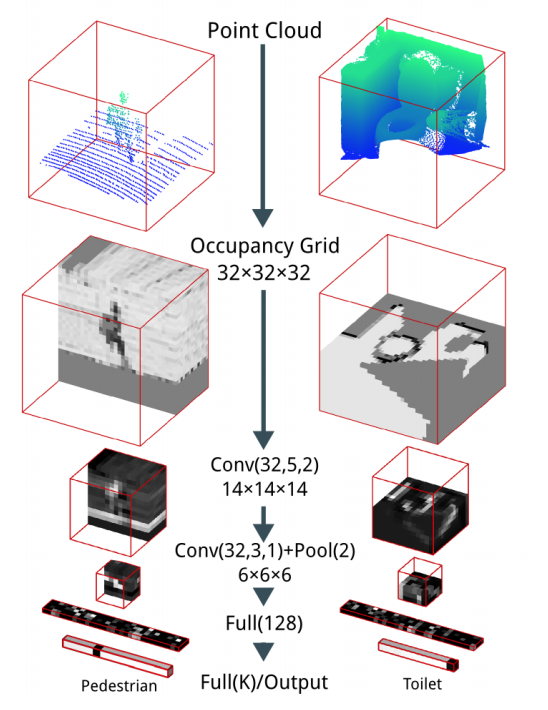
\includegraphics[scale=0.25]{Images/Chapter 3/voxelgrid.png}
    \caption{Voxel Grid example: A 3D Convolutional Neural Network for Real-Time Object Recognition}
    \label{fig:voxel}
\end{figure}


\textbf{T265 Intel Tracking Camera}

The T265 tracking camera is designed to integrate odometry data from the robot. It is in fact an independent and robust support for visual-inertia odometry and re-localisation.
A key strength of visual-inertial odometry is that the various sensors available complement each other. The images from the visual sensors are supplemented by data from an onboard inertial measurement unit (IMU), which includes a gyroscope and accelerometer. The aggregated data from these sensors is fed into simultaneous localization and mapping (SLAM) algorithms.
The tracking is done by comparing the information collected by the two fish-eye cameras, which collect images at 30 fps, \citet{inteltracking}.
\begin{figure}[H]
    \centering
    \begin{subfigure}
            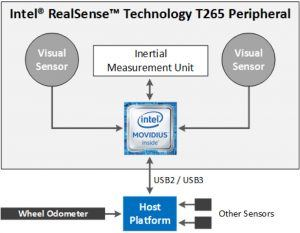
\includegraphics[scale=0.5]{Images/Chapter 3/t265diagram.jpg}
    \caption{Block diagram of Intel T265}
    \label{fig:t265block}
    \end{subfigure}%
    ~
    \begin{subfigure}
        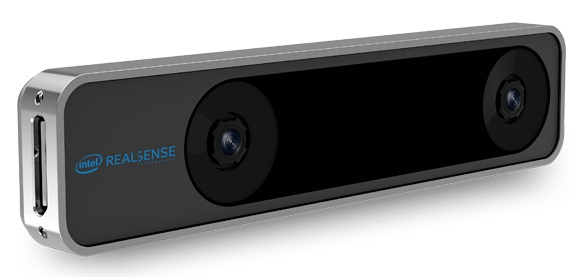
\includegraphics[scale=0.5]{Images/Chapter 3/t265.jpg}
        \caption{T265 Intel Tracking Camera }
        \label{fig:t265}
    \end{subfigure}
\end{figure}

\textbf{YDLidar}

LiDAR (Light Detection And Ranging) identifies technology that measures the distance to an object by illuminating it with laser light, while at the same time being able to return high-resolution three-dimensional information about the surrounding environment. A LiDAR typically uses several components: lasers, photodetectors and readout integrated circuits (ROICs) with time-of-flight (TOF) capability to measure distance by illuminating a target and analysing the reflected light.
\begin{figure}[H]
    \centering
    \begin{subfigure}
            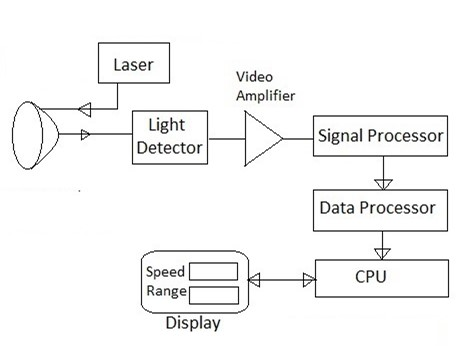
\includegraphics[scale=0.7]{Images/Chapter 3/lidar.jpg}
            \caption{Lidar scheme}
            \label{fig:lidarscheme}
        \end{subfigure}
    \begin{subfigure}
            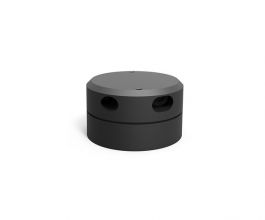
\includegraphics{Images/Chapter 3/ydlidar.jpg}
            \caption{YDLidar }
            \label{fig:ydlidar}
    \end{subfigure}
\end{figure}
YDLIDAR G2 is a 360-degree two-dimensional rangefinder 
developed by YDLIDAR. Based on the principle of triangulation, it is equipped withrelatedoptics, electricity, and algorithm design to achieve high-frequency and high-precision distancemeasurement. The mechanical structure rotates 360 degrees to continuously output the angle information as well as the point cloud data of the scanning environment while ranging.

\subsubsection{Visual Fiducial System}
During the use and development of Robee's navigation, so-called Apriltags were used, a particular visual fiducial system chosen for its robustness and integration with the simulated Gazebo environment.
Visual fiducials are nothing more than artificial landmarks, designed to be easily recognisable within the working environment and distinguishable from one another.
The methodology is similar to that of a common QR code but with significant applications and objectives.
In fact, unlike a QR code, where the user has to frame the tag with the camera and capture the high-resolution snapshot, these types of tags are designed to work with a small amount of information (even as little as 12 bits) but with performance and ease of use that is clearly superior to QR codes. In fact, these types of tags are designed to be automatically detectable and localisable even in low resolution conditions, even providing the relative position and orientation of the tag with respect to the camera.
In terms of size, the Apriltags used range from 50 to 100 pixels, including the payload, \citet{olson2011tags}.
\begin{figure}[H]
    \centering
    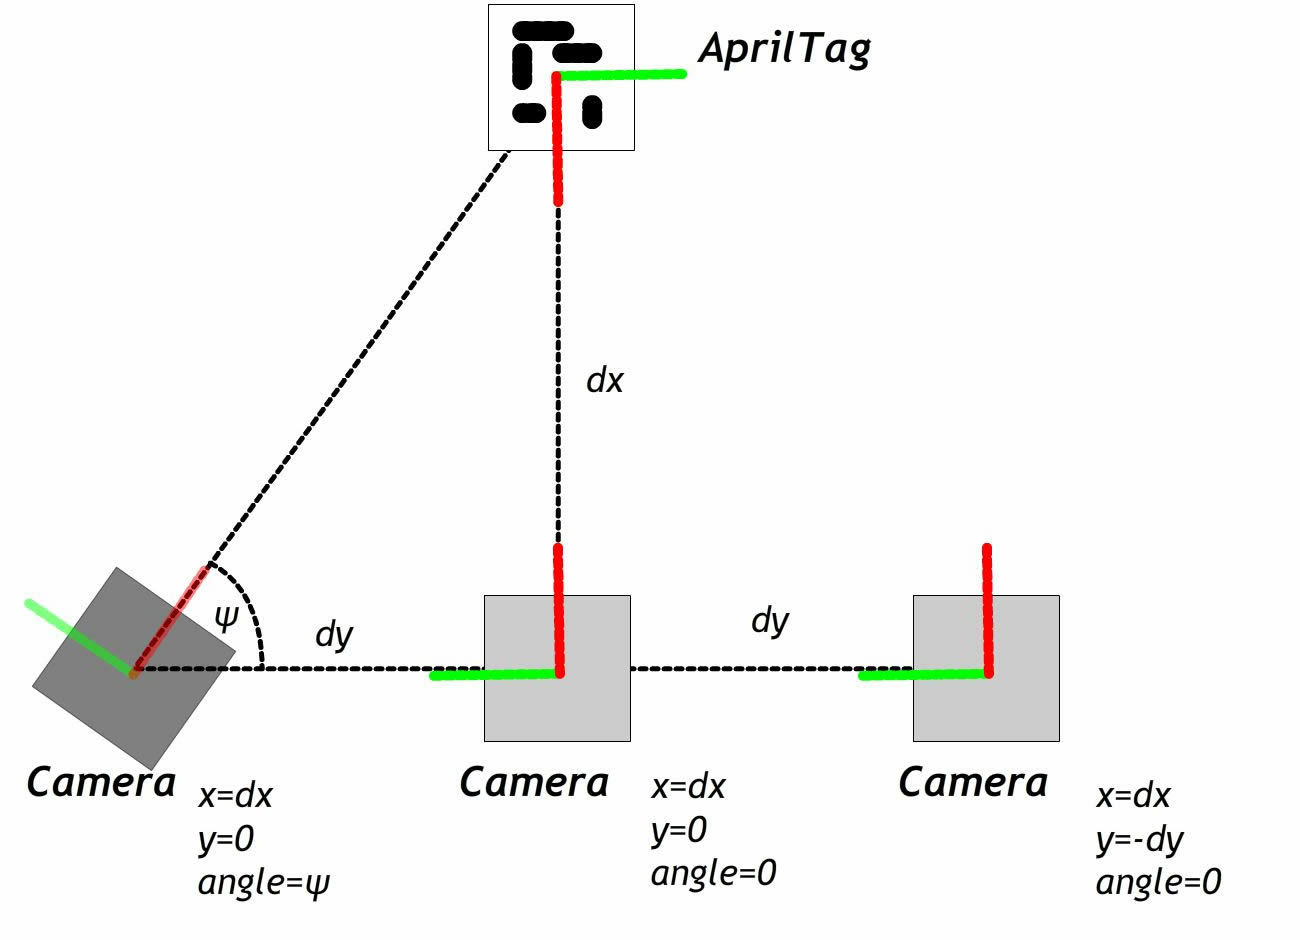
\includegraphics[scale=0.25]{Images/Chapter 3/apriltag.jpg}
    \caption{AprilTag distance and orientation measurement}
    \label{fig:apriltag}
\end{figure}

\begin{figure}[H]
    \centering
    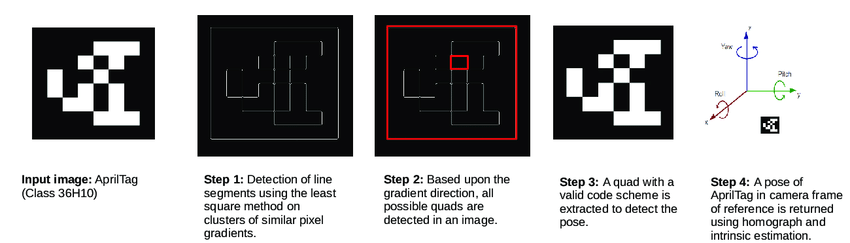
\includegraphics[scale=0.6]{Images/Chapter 3/apriltagsteps.png}
    \caption{How AprilTag detection is performed}
    \label{fig:apriltagsteps}
\end{figure}
Visual fiducial systems have been used in robotics to improve human/machine interaction, enabling the development of commands such as 'follow me'.
In the context of this work, tags were used for SLAM (Simultaneous Localisation and Mapping), as an independent support to the sensors mentioned in the previous section.
In fact, in both the simulated and real environment, tags were placed in strategic positions in order to reposition the robot to the correct pose by comparing the information coming from the sensors and that coming from the tags.
AprilTag provides a package for perfect ROS integration.
\begin{figure}[H]
    \centering
    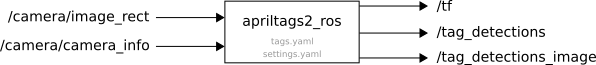
\includegraphics{Images/Chapter 3/aprilros.png}
    \caption{ROS TF}
    \label{fig:aprilros}
\end{figure}

The apriltag ROS package then takes as input the topic of the rectified image and returns a list of recognised tags and their positions in 3 dimensions.
However, in order to work, one must specify in the configuration files (settings and tags) which tag families to search for.
A practical application will be provided in chapter \ref{ch:sim_test}

\subsubsection{Indoor Positioning System}

For the purpose of this thesis, another technology that has been used is the Indoor Positioning System.
This is in fact a new approach to the problem of localisation when remote GNSS satellites, which are commonly blocked indoors, are not available.
There is now a wide offer for this type of solution, even with different communication protocols at its base: from Wi-Fi signals to Bluetooth to ultrasound.
In Robee, the choice was made to use an IPS system provided by Marvelmind, which is based on ultrasonic and time-of-flight (ToF) measurements with trilateration and which also provides for communication via ROS topics, thus providing integration with the robotics platform used.
The system proposed by Marvelmind consists of a series of static beacons (four were used in our case), placed on the walls of the production area of Oversonic Robotics.

\begin{figure}[H]
    \centering
    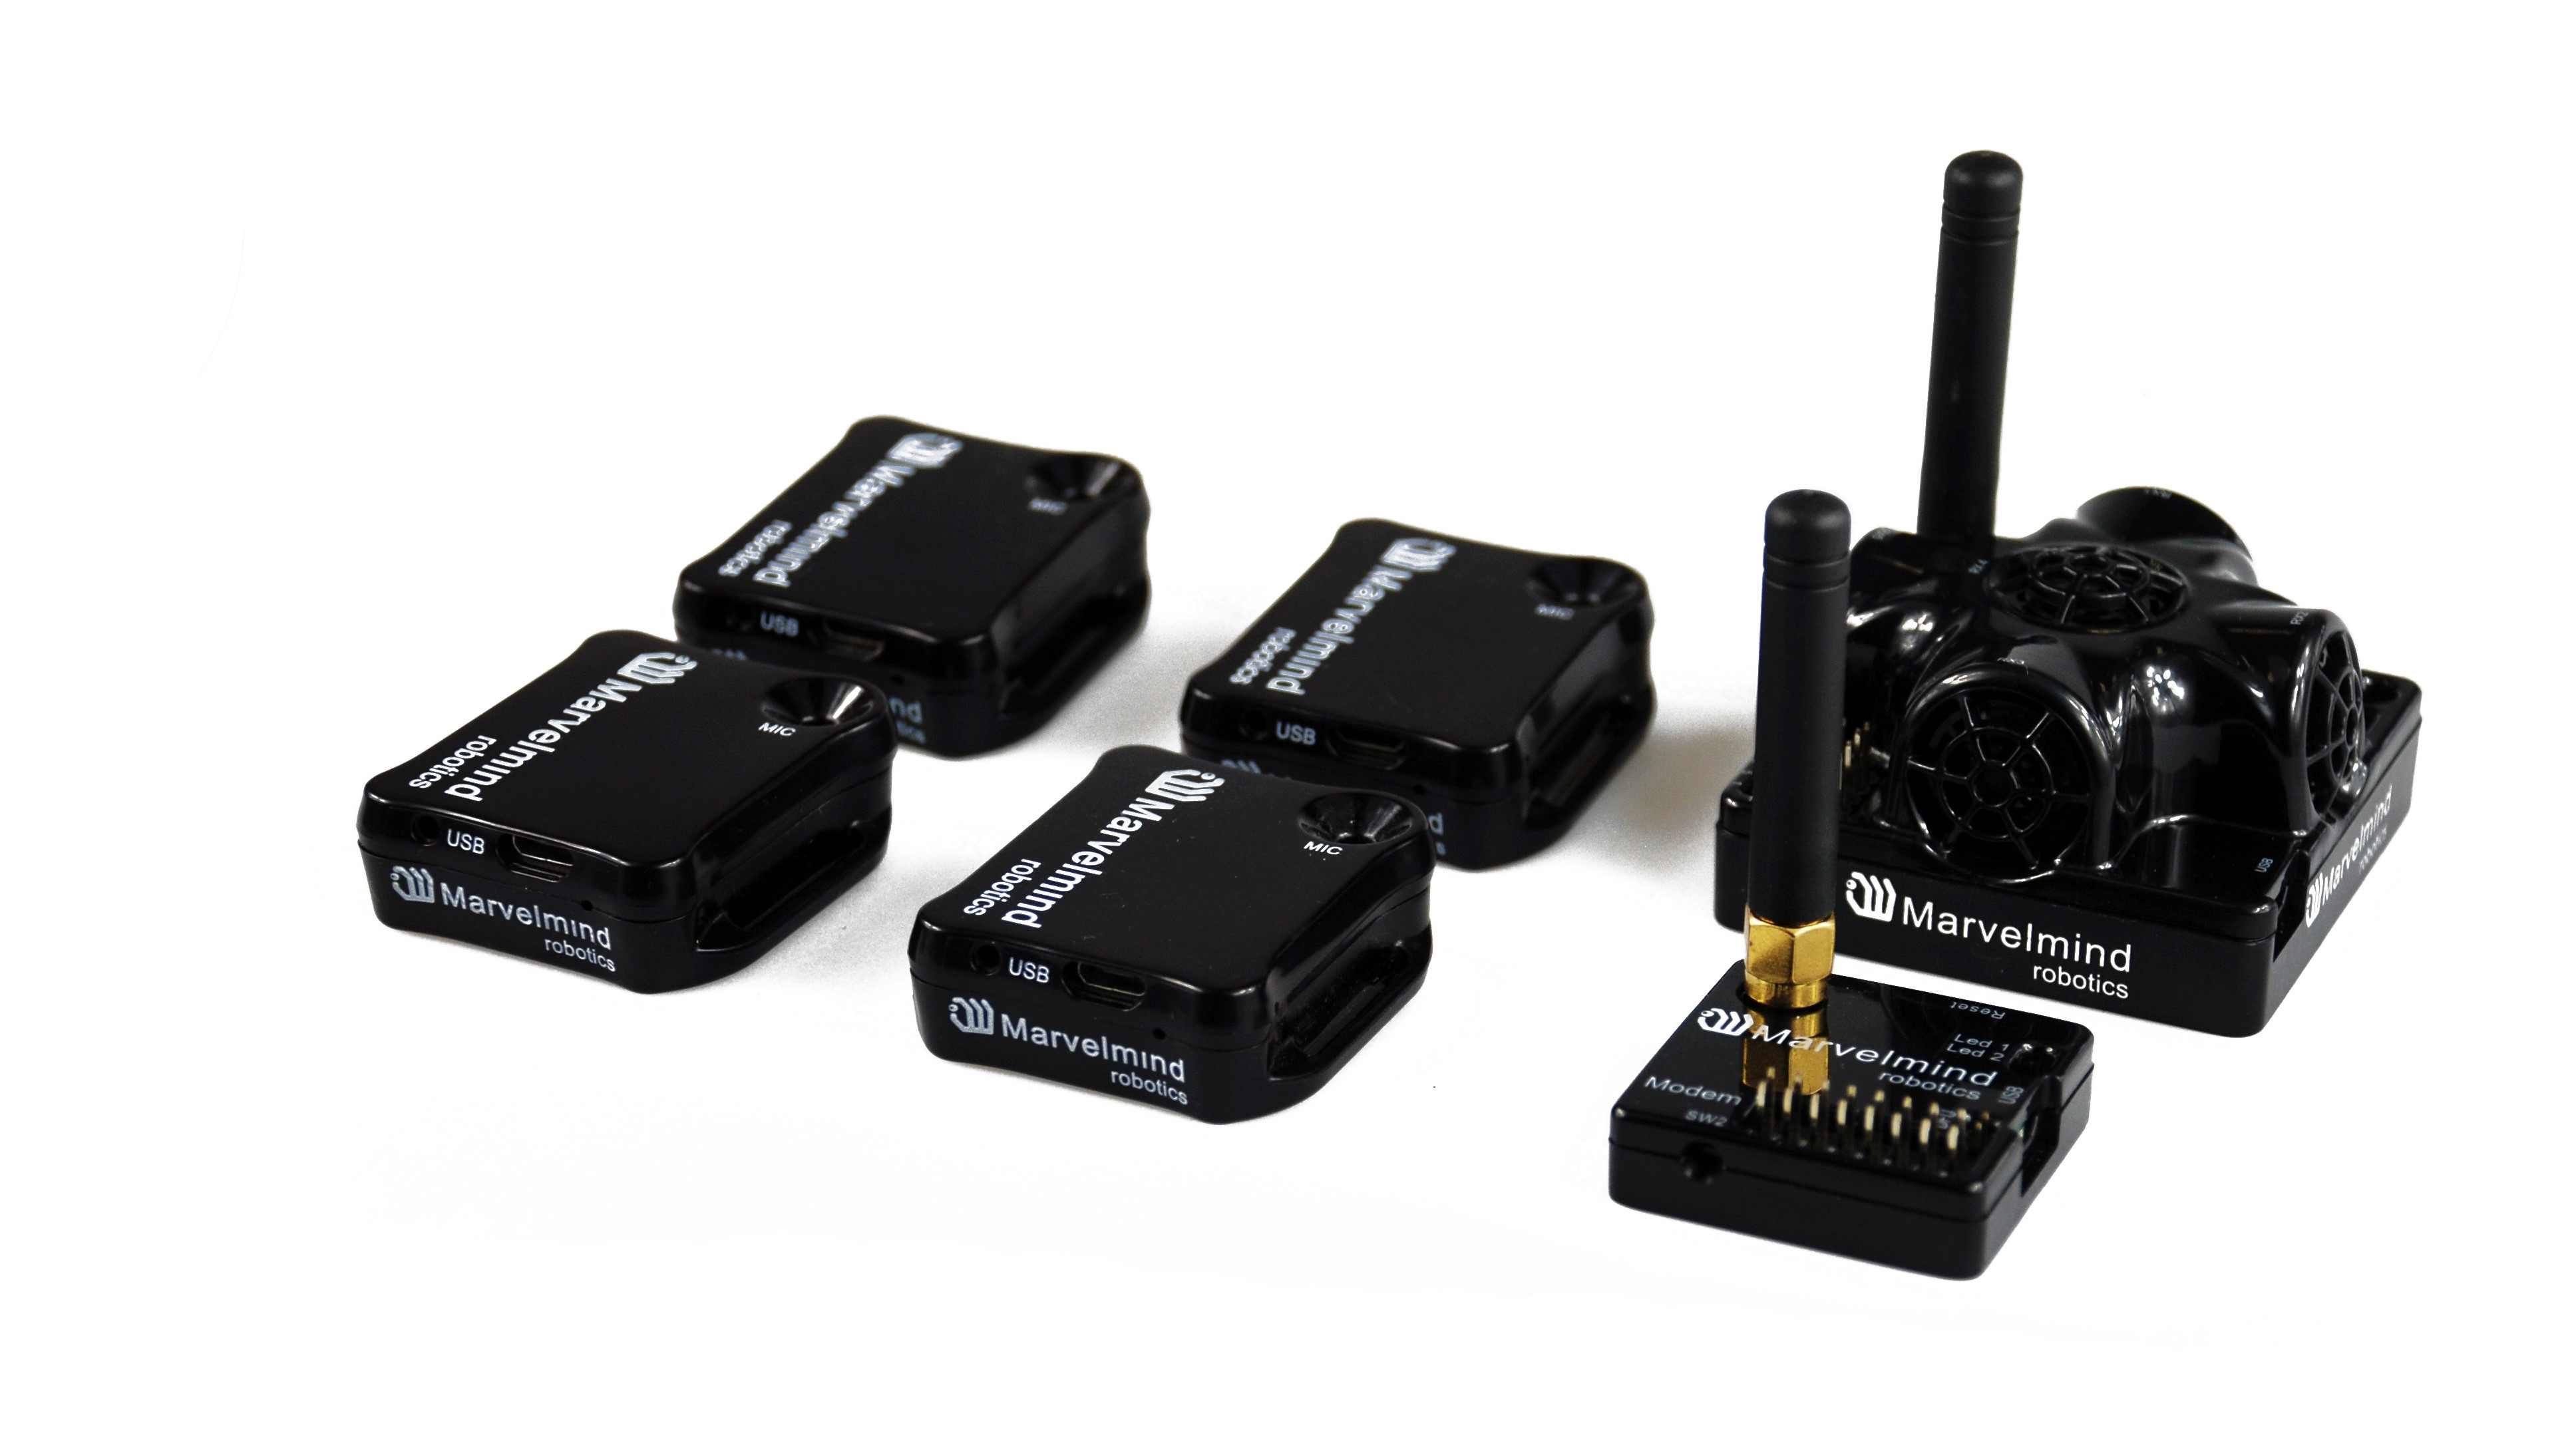
\includegraphics[scale=0.25]{Images/Chapter 3/beacon.jpg}
    \caption{MarvelMind beacons kit}
    \label{fig:beacon}
\end{figure}

Each beacon sends and receives a stream of hypersonic signals continuously. There is also a modem, which is connected to the PC on which the supplied software is run, and a beacon called a 'hedgehog' which is placed on the vehicle to be located, in this case Robee. The hedgehog then receives the signals from the four beacons and sends them to the modem, which proceeds to triangulate.
The communication frequency is customisable and directly affects localisation accuracy, which in the basic configuration is claimed to be +/- 2 cm.



\chapter{Conclusions and future developments}
\label{ch:conclusions}%
A final chapter containing the main conclusions of your research/study
and possible future developments of your work have to be inserted in this chapter.

%-------------------------------------------------------------------------
%	BIBLIOGRAPHY
%-------------------------------------------------------------------------

\addtocontents{toc}{\vspace{2em}} % Add a gap in the Contents, for aesthetics
\bibliography{Thesis_bibliography} % The references information are stored in the file named "Thesis_bibliography.bib"

%-------------------------------------------------------------------------
%	APPENDICES
%-------------------------------------------------------------------------

\cleardoublepage
\addtocontents{toc}{\vspace{2em}} % Add a gap in the Contents, for aesthetics
\appendix
\chapter{Appendix A}
If you need to include an appendix to support the research in your thesis, you can place it at the end of the manuscript.
An appendix contains supplementary material (figures, tables, data, codes, mathematical proofs, surveys, \dots)
which supplement the main results contained in the previous chapters.

\chapter{Appendix B}
It may be necessary to include another appendix to better organize the presentation of supplementary material.


% LIST OF FIGURES
\listoffigures

% LIST OF TABLES
\listoftables

% LIST OF SYMBOLS
% Write out the List of Symbols in this page
\chapter*{List of Symbols} % You have to include a chapter for your list of symbols (
\begin{table}[H]
    \centering
    \begin{tabular}{lll}
        \textbf{Variable} & \textbf{Description} & \textbf{SI unit} \\\hline\\[-9px]
        $\bm{u}$ & solid displacement & m \\[2px]
        $\bm{u}_f$ & fluid displacement & m \\[2px]
    \end{tabular}
\end{table}

% ACKNOWLEDGEMENTS
\chapter*{Acknowledgements}
Here you might want to acknowledge someone.

\cleardoublepage

\end{document}
